\bibliography{../References/refer}

\section{Analysis}
	\label{sec:Analysis}
	So we have established the details of the differences between the different variations of quicksorts.
	To investigate and compare the algorithms we have implemented and ran experiments. 
	We used uniformly random numbers from $0$ to $10^{12}$.
	Then created arrays with randomly generated integers for sizes $4$ to $50$ million
	Table \ref{tab:FullSortList} shows the variations of quicksort to the arrays generated.
	\begin{table}
		\begin{center}
			\begin{tabular}{|r|c|c|}
				\hline
				Name of Sort Algorithm           & Pivot Selection Methods & Number of Pivots \\ \hline \hline
				Classic Quicksort                &  3  &  1       \\ \hline
				Dual Pivot Quicksort             &  2  &  2       \\ \hline
				Heap Optimized M-Pivot Quicksort &  1  &  3,4,5,6 \\ \hline
				M-Pivot Quicksort                &  1  &  3,4,5,6 \\ \hline
				Optimal Dual Pivot Quicksort     &  2  &  2       \\ \hline
				Three Pivot Quicksort            &  1  &  3       \\ \hline
				Yaroslavskiy Quicksort           &  1  &  2       \\ \hline
			\end{tabular}
			\caption{List of all the variation of quicksorts executed.}
			\label{tab:FullSortList}
		\end{center}
	\end{table}


	%**********************************************************************
	% Determine if we need to talk about pivot selection here
	%**********************************************************************
	%The pivot selection methods differ by which quicksort algorithm we are referring too.
	%For the classic quick sort algorithm, 
	%the pivot selection method $1$ and $2$ would refer to picking the first or last element as the pivot respectively.
	%Pivot selection method $3$ refers to picking the median of 3 elements.
	%Which these would be the one of the first, middle, or last element.
	%For dual pivot and optimal dual pivot, pivot selection $1$ refers

	Figure \ref{fig:PlotLegend} is the legend of all the plots generated.
	You can see the color and shape combination for each version of quick sort algorithm. 
	These color and shape choices will be consistent throughout the following plots.
	There are 17 distinct derivatives of quicksort that have been run.
	Note that for the plots we overlay the function :
	\begin{equation}
		A\cdot n\log(n) + B\cdot n + C \log(n)
		\label{eq:FitFunction}
	\end{equation}
	The nomenclature for the legend is as follows: 
	\begin{center}
		(Algorithm Name, Pivot Selection Method Index, Number of Pivots, is Insertion Sort used).
	\end{center}

	\begin{figure}[ht!]
		\begin{center}   
			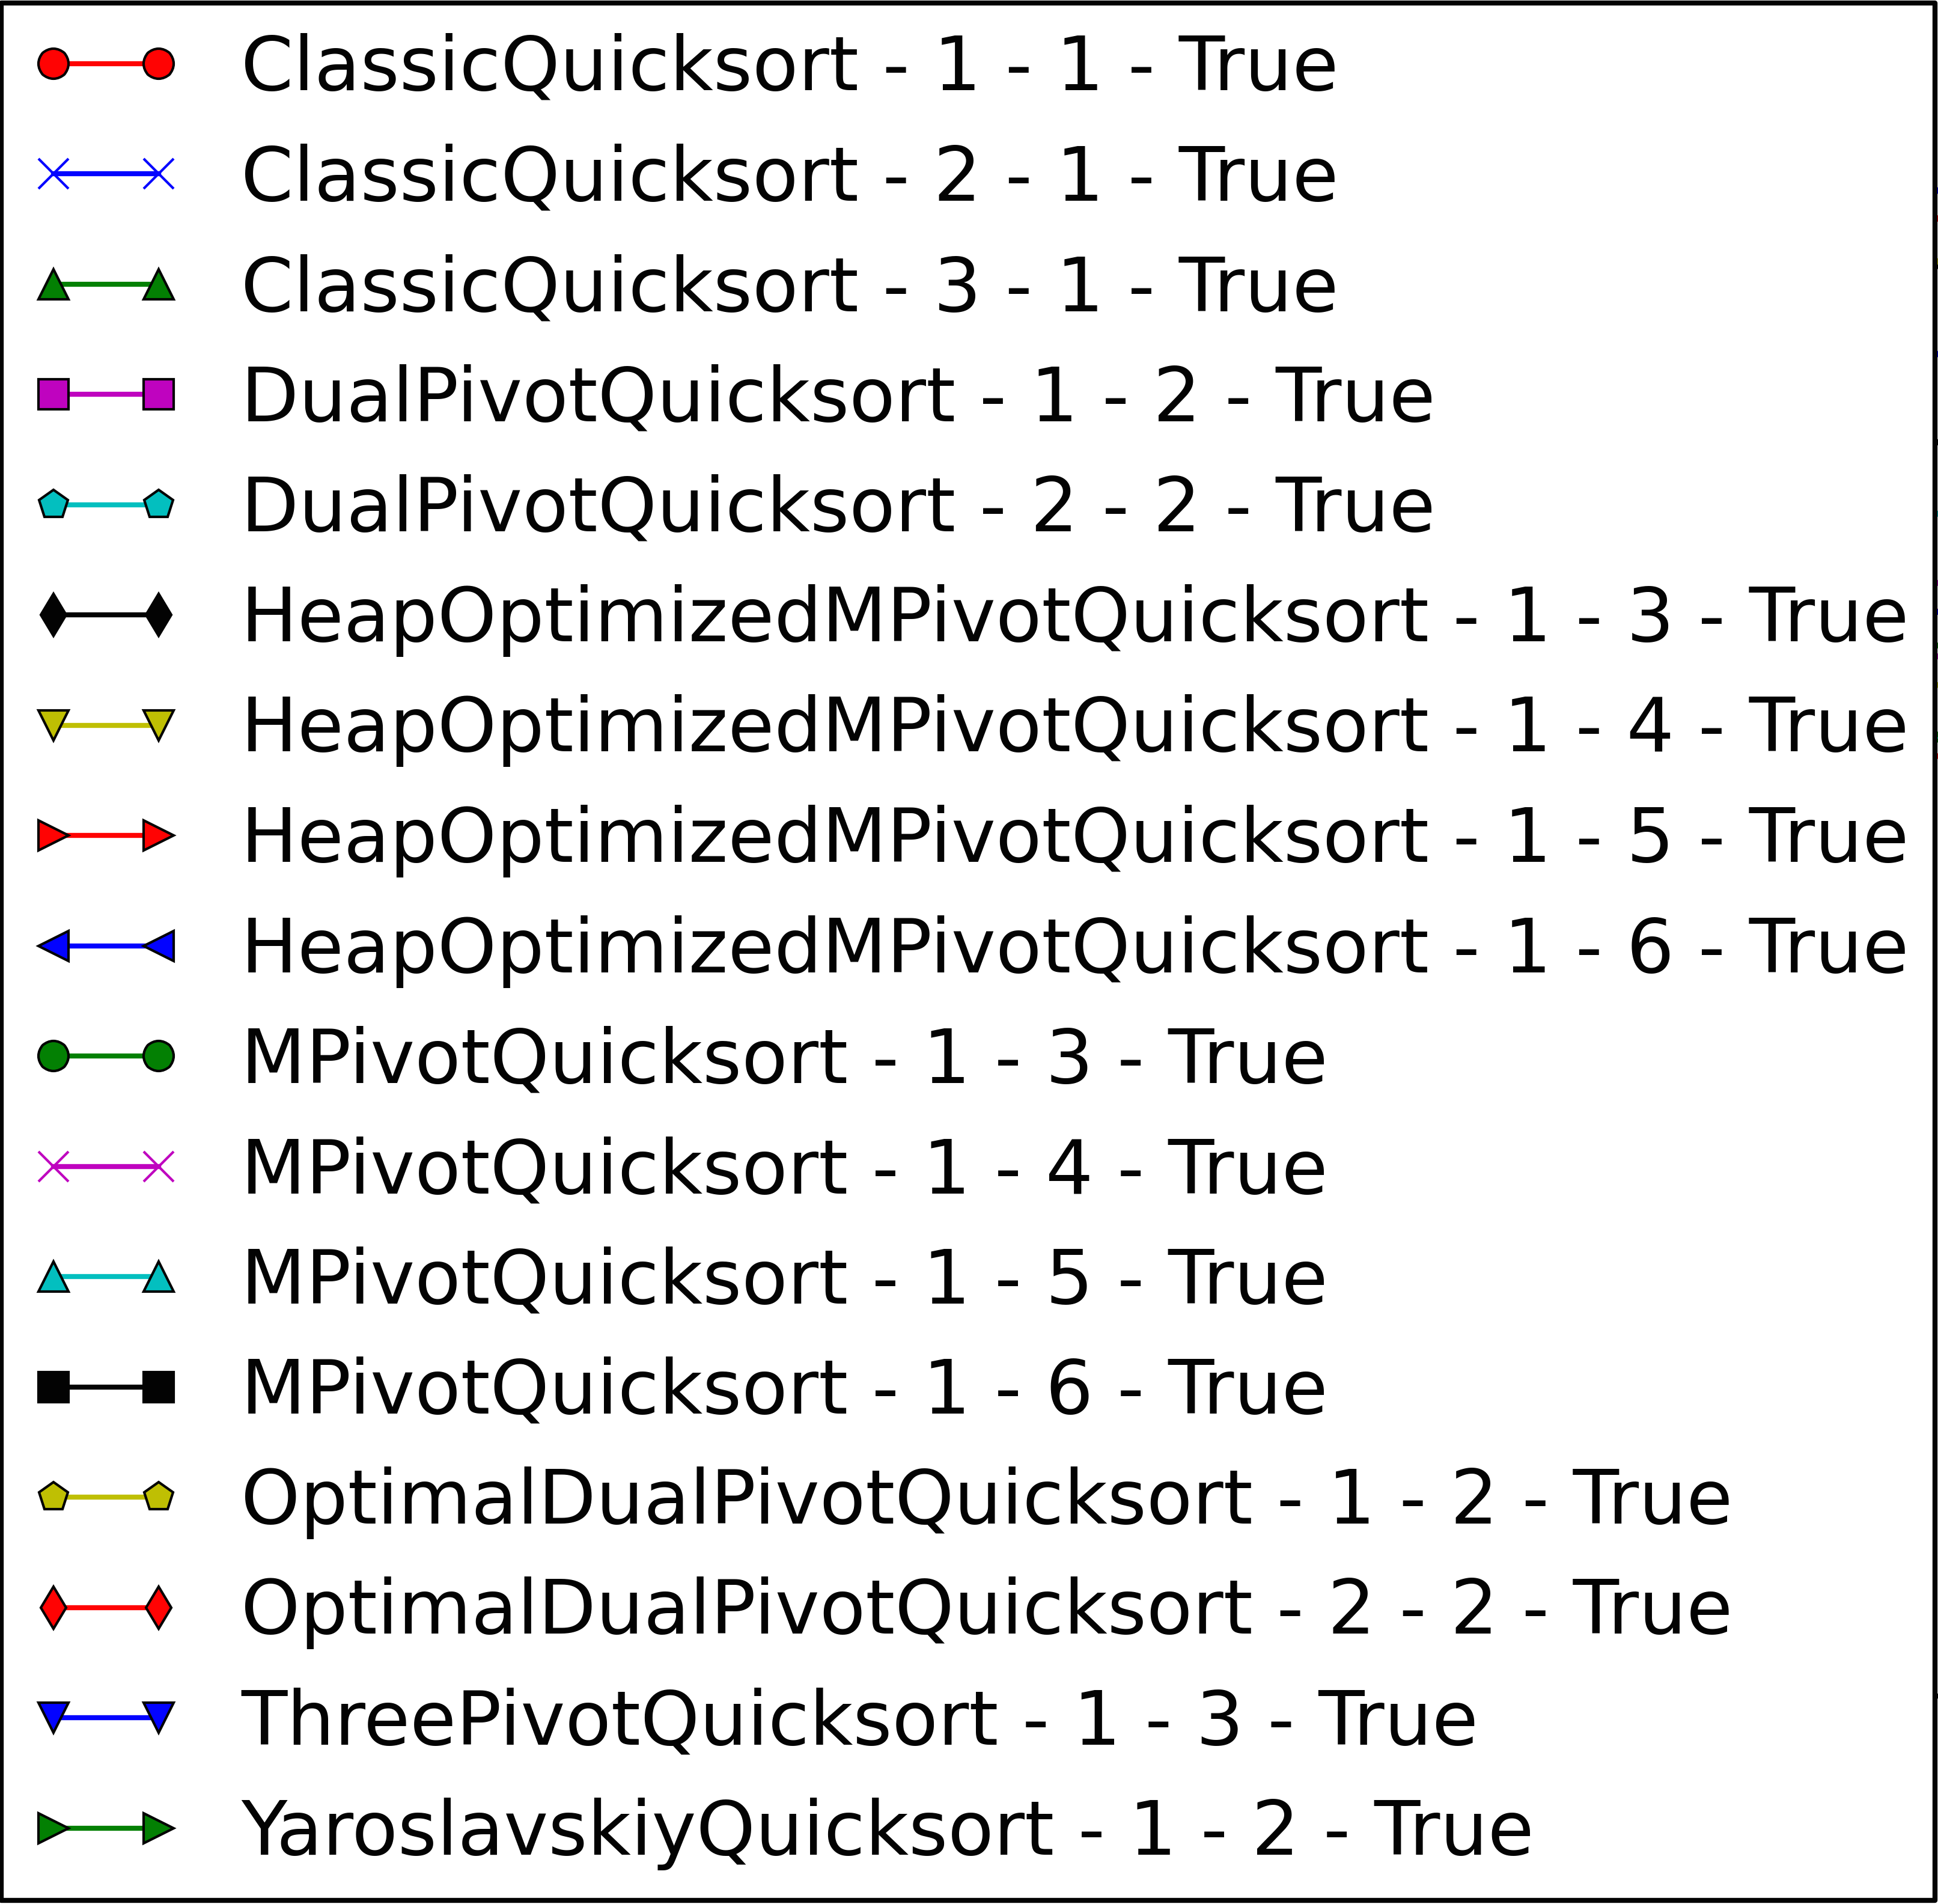
\includegraphics[width=85mm]{PlotLegend.png}
			\label{fig:PlotLegend}
			\caption{A visual reference for all the quicksort variations and plots.}
		\end{center}
	\end{figure}

	\subsection{Data Processing}
		\label{subsec:DataProcessing}
		In processing the data, we take averages of any common data entries. We plot them and have the following results.
		Which is summarized in Figures \ref{fig:AllSorts}, \ref{fig:TwoPivot}, \ref{fig:ThreePivot}, and \ref{fig:MPivot}.

		%**********************************************************************
		% All Plots Large Scale
		%**********************************************************************
		\begin{figure}[ht!]
			\begin{center}
				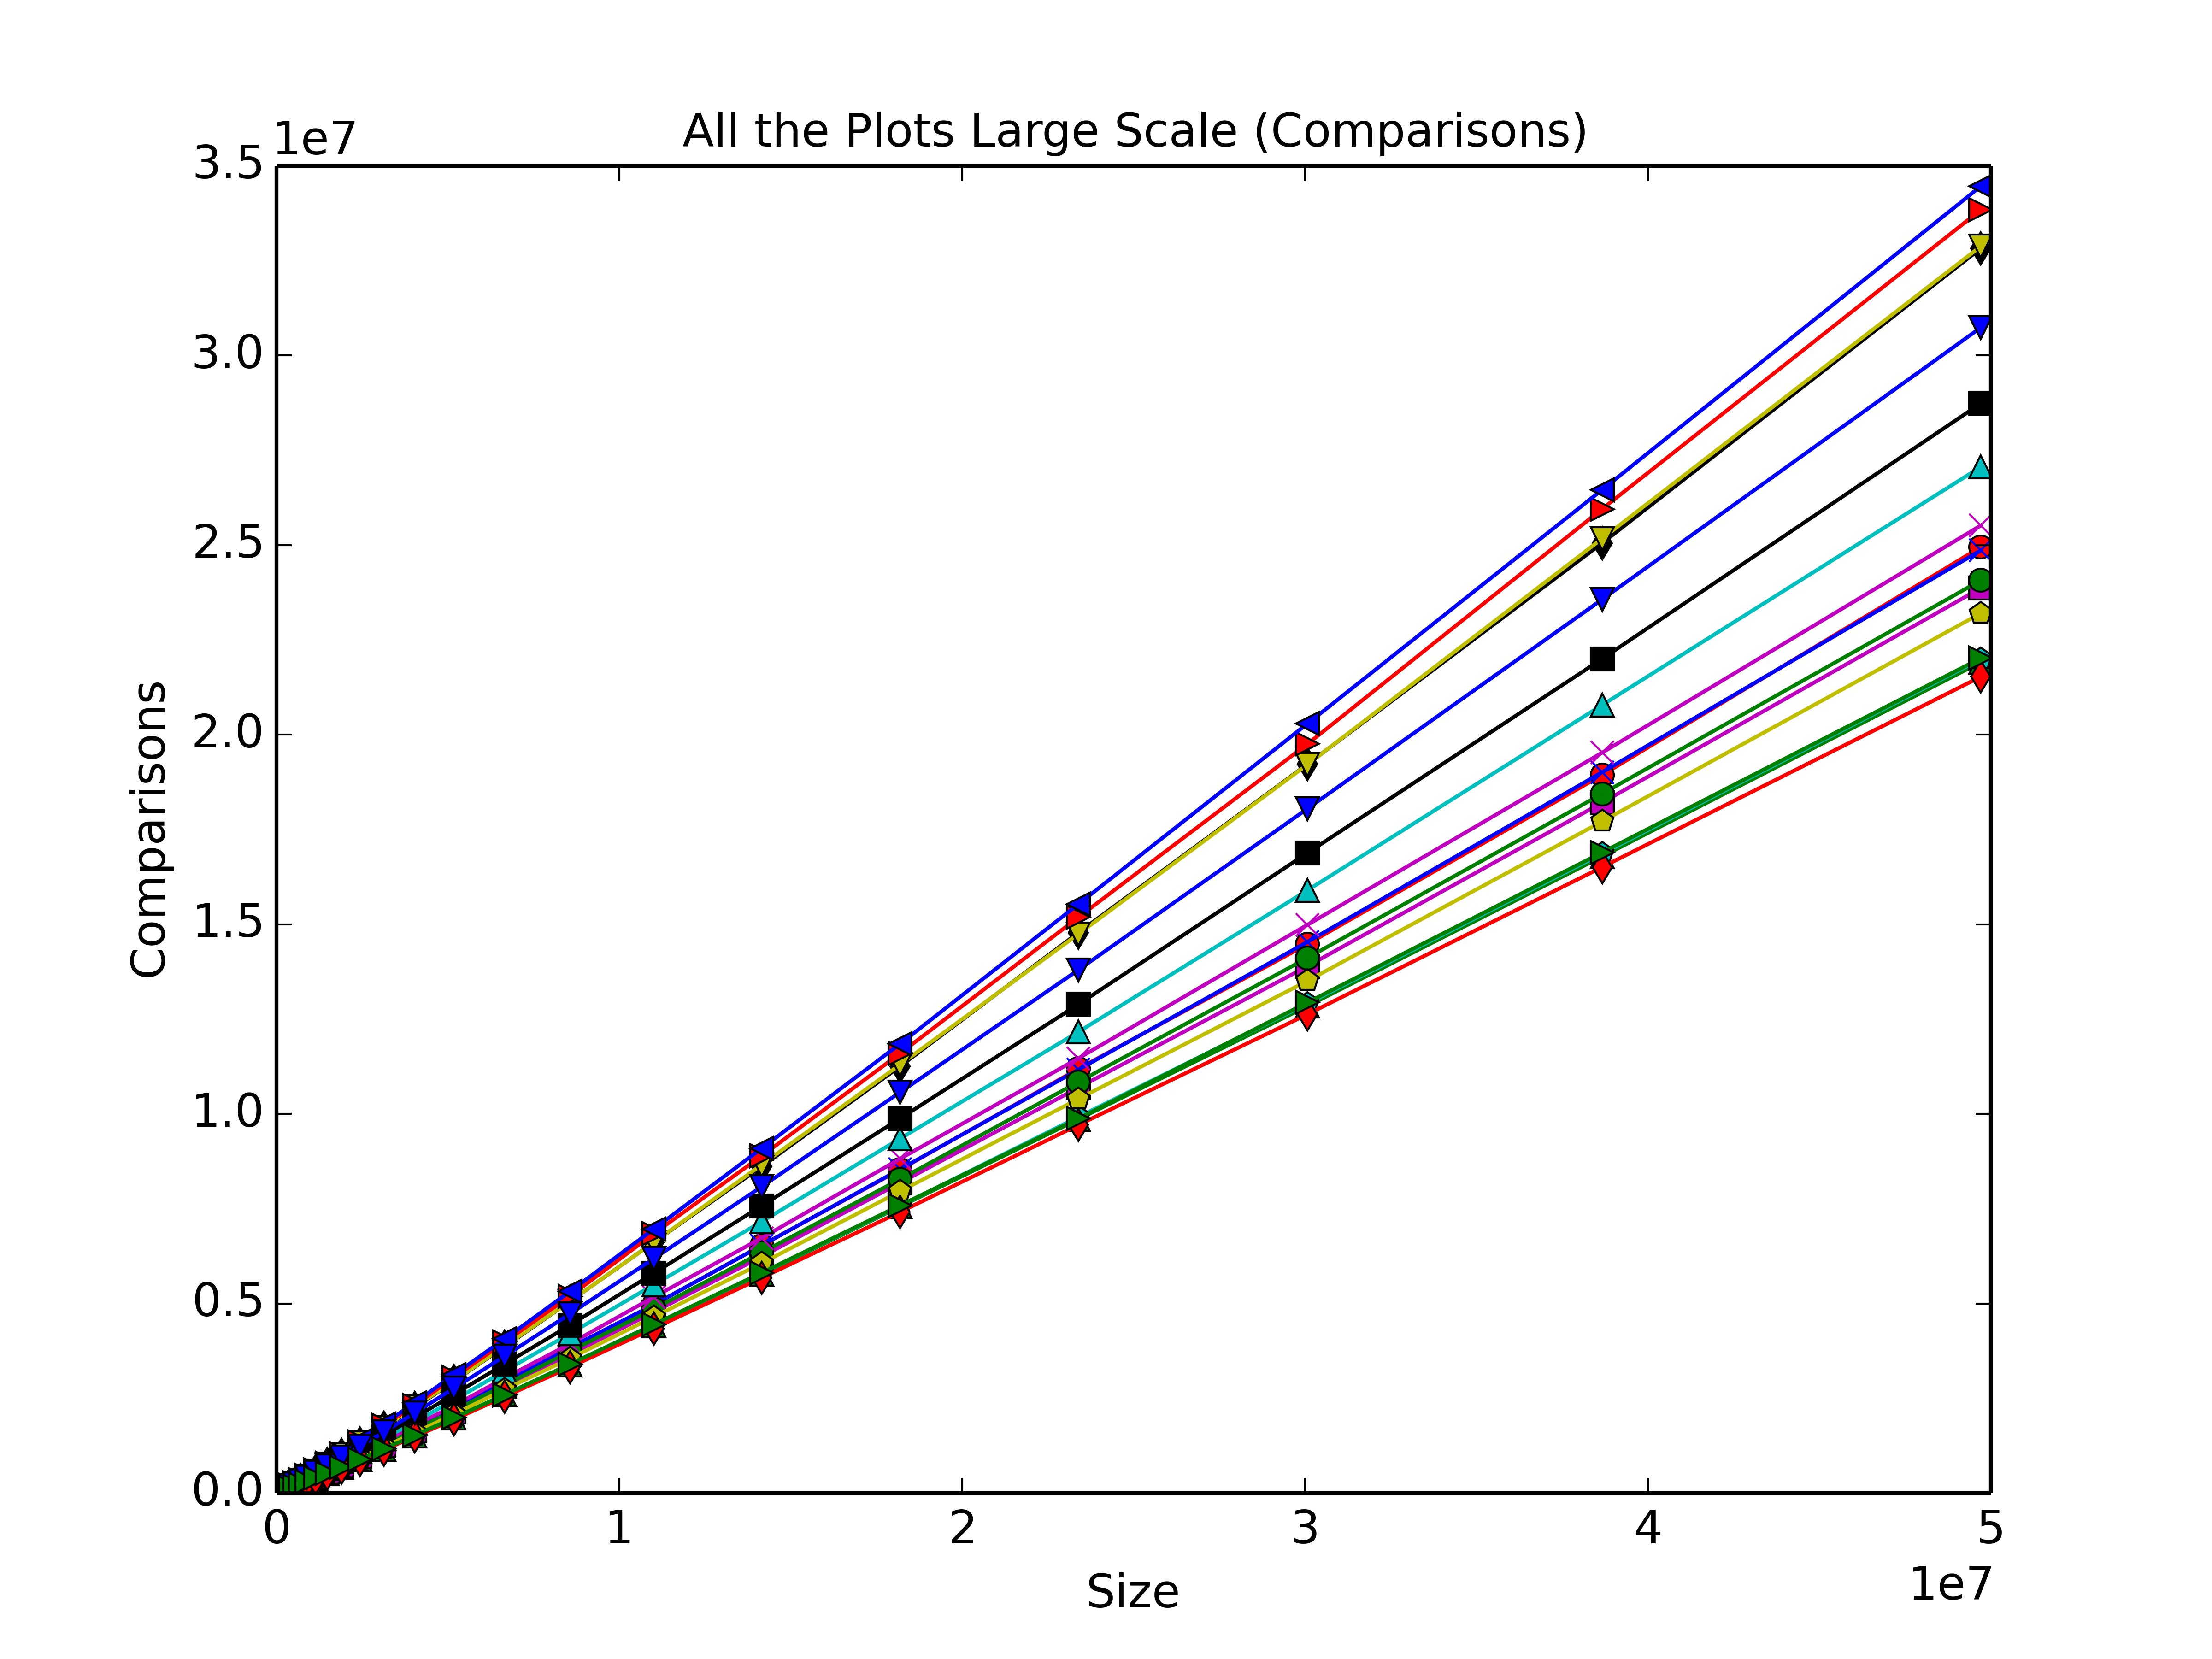
\includegraphics[width=150mm]{AllthePlotsLargeScale_comp}
				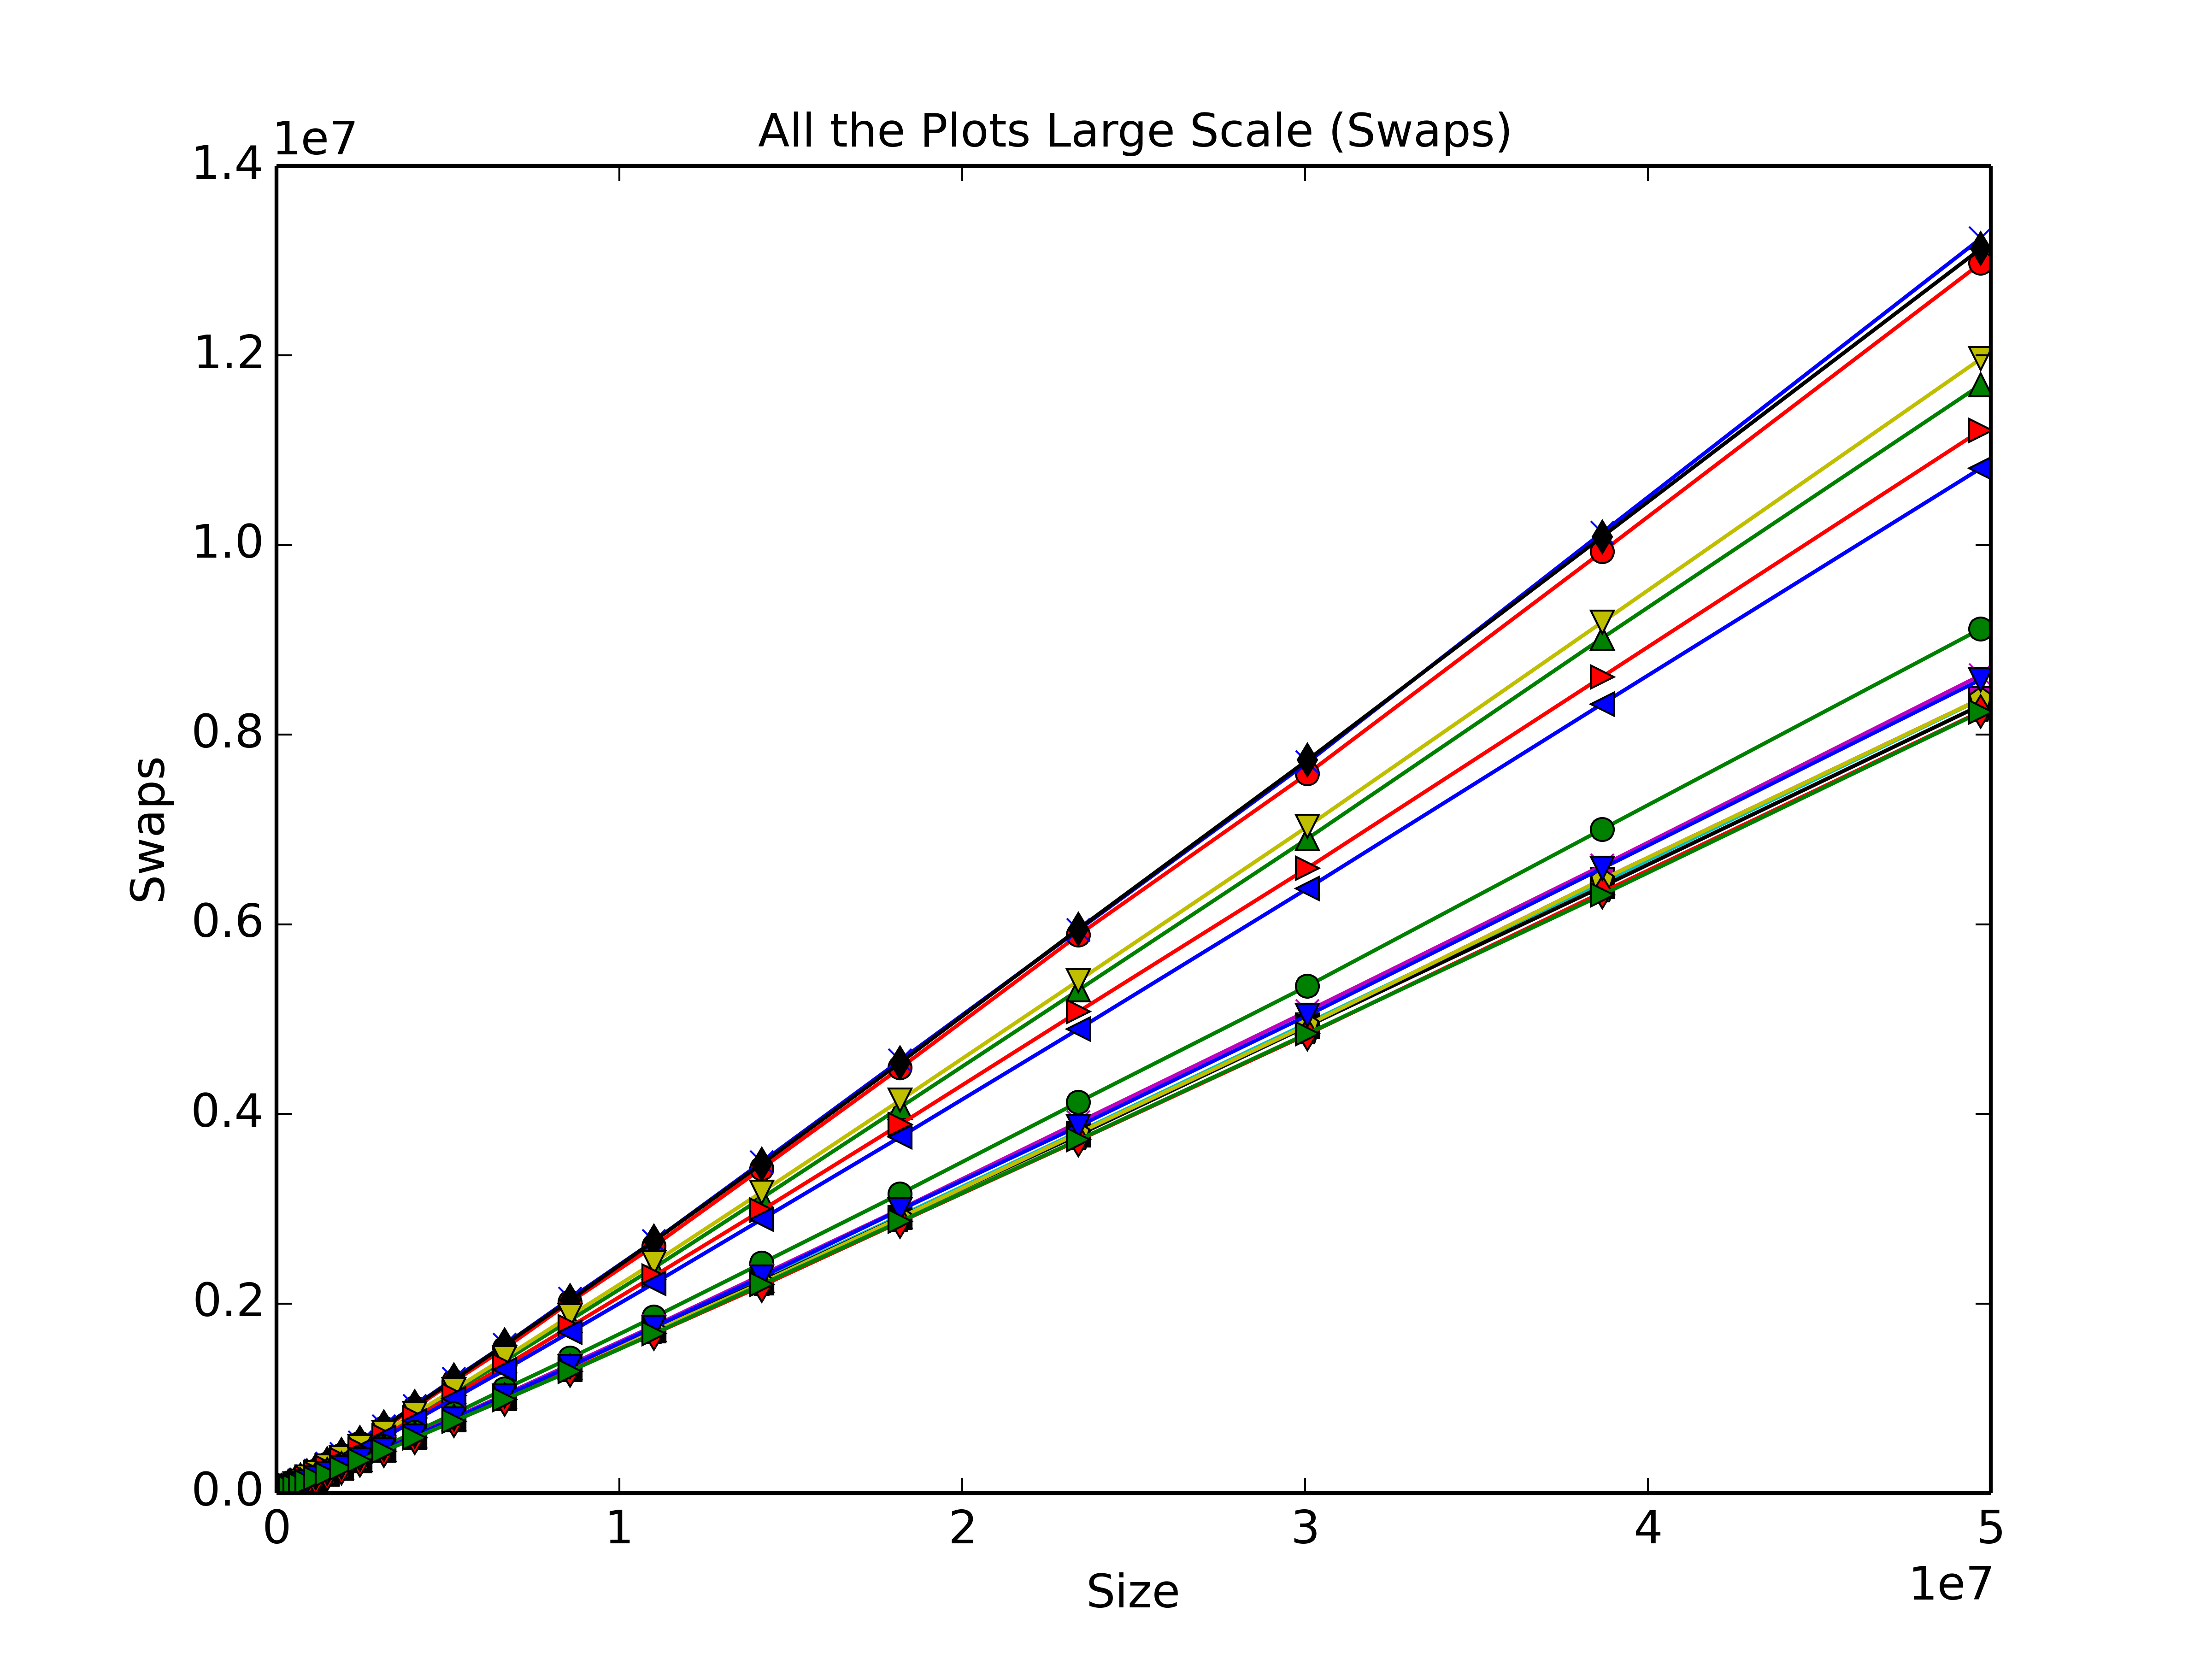
\includegraphics[width=150mm]{AllthePlotsLargeScale_swap}
				\caption{A plot of the data from all the sorting algorithm against the number of comparisons.}
				\label{fig:AllSorts}
			\end{center}
		\end{figure}


		%**********************************************************************
		% All Plots Log Large Scale
		%**********************************************************************
		\begin{figure}[ht!]
			\begin{center}
				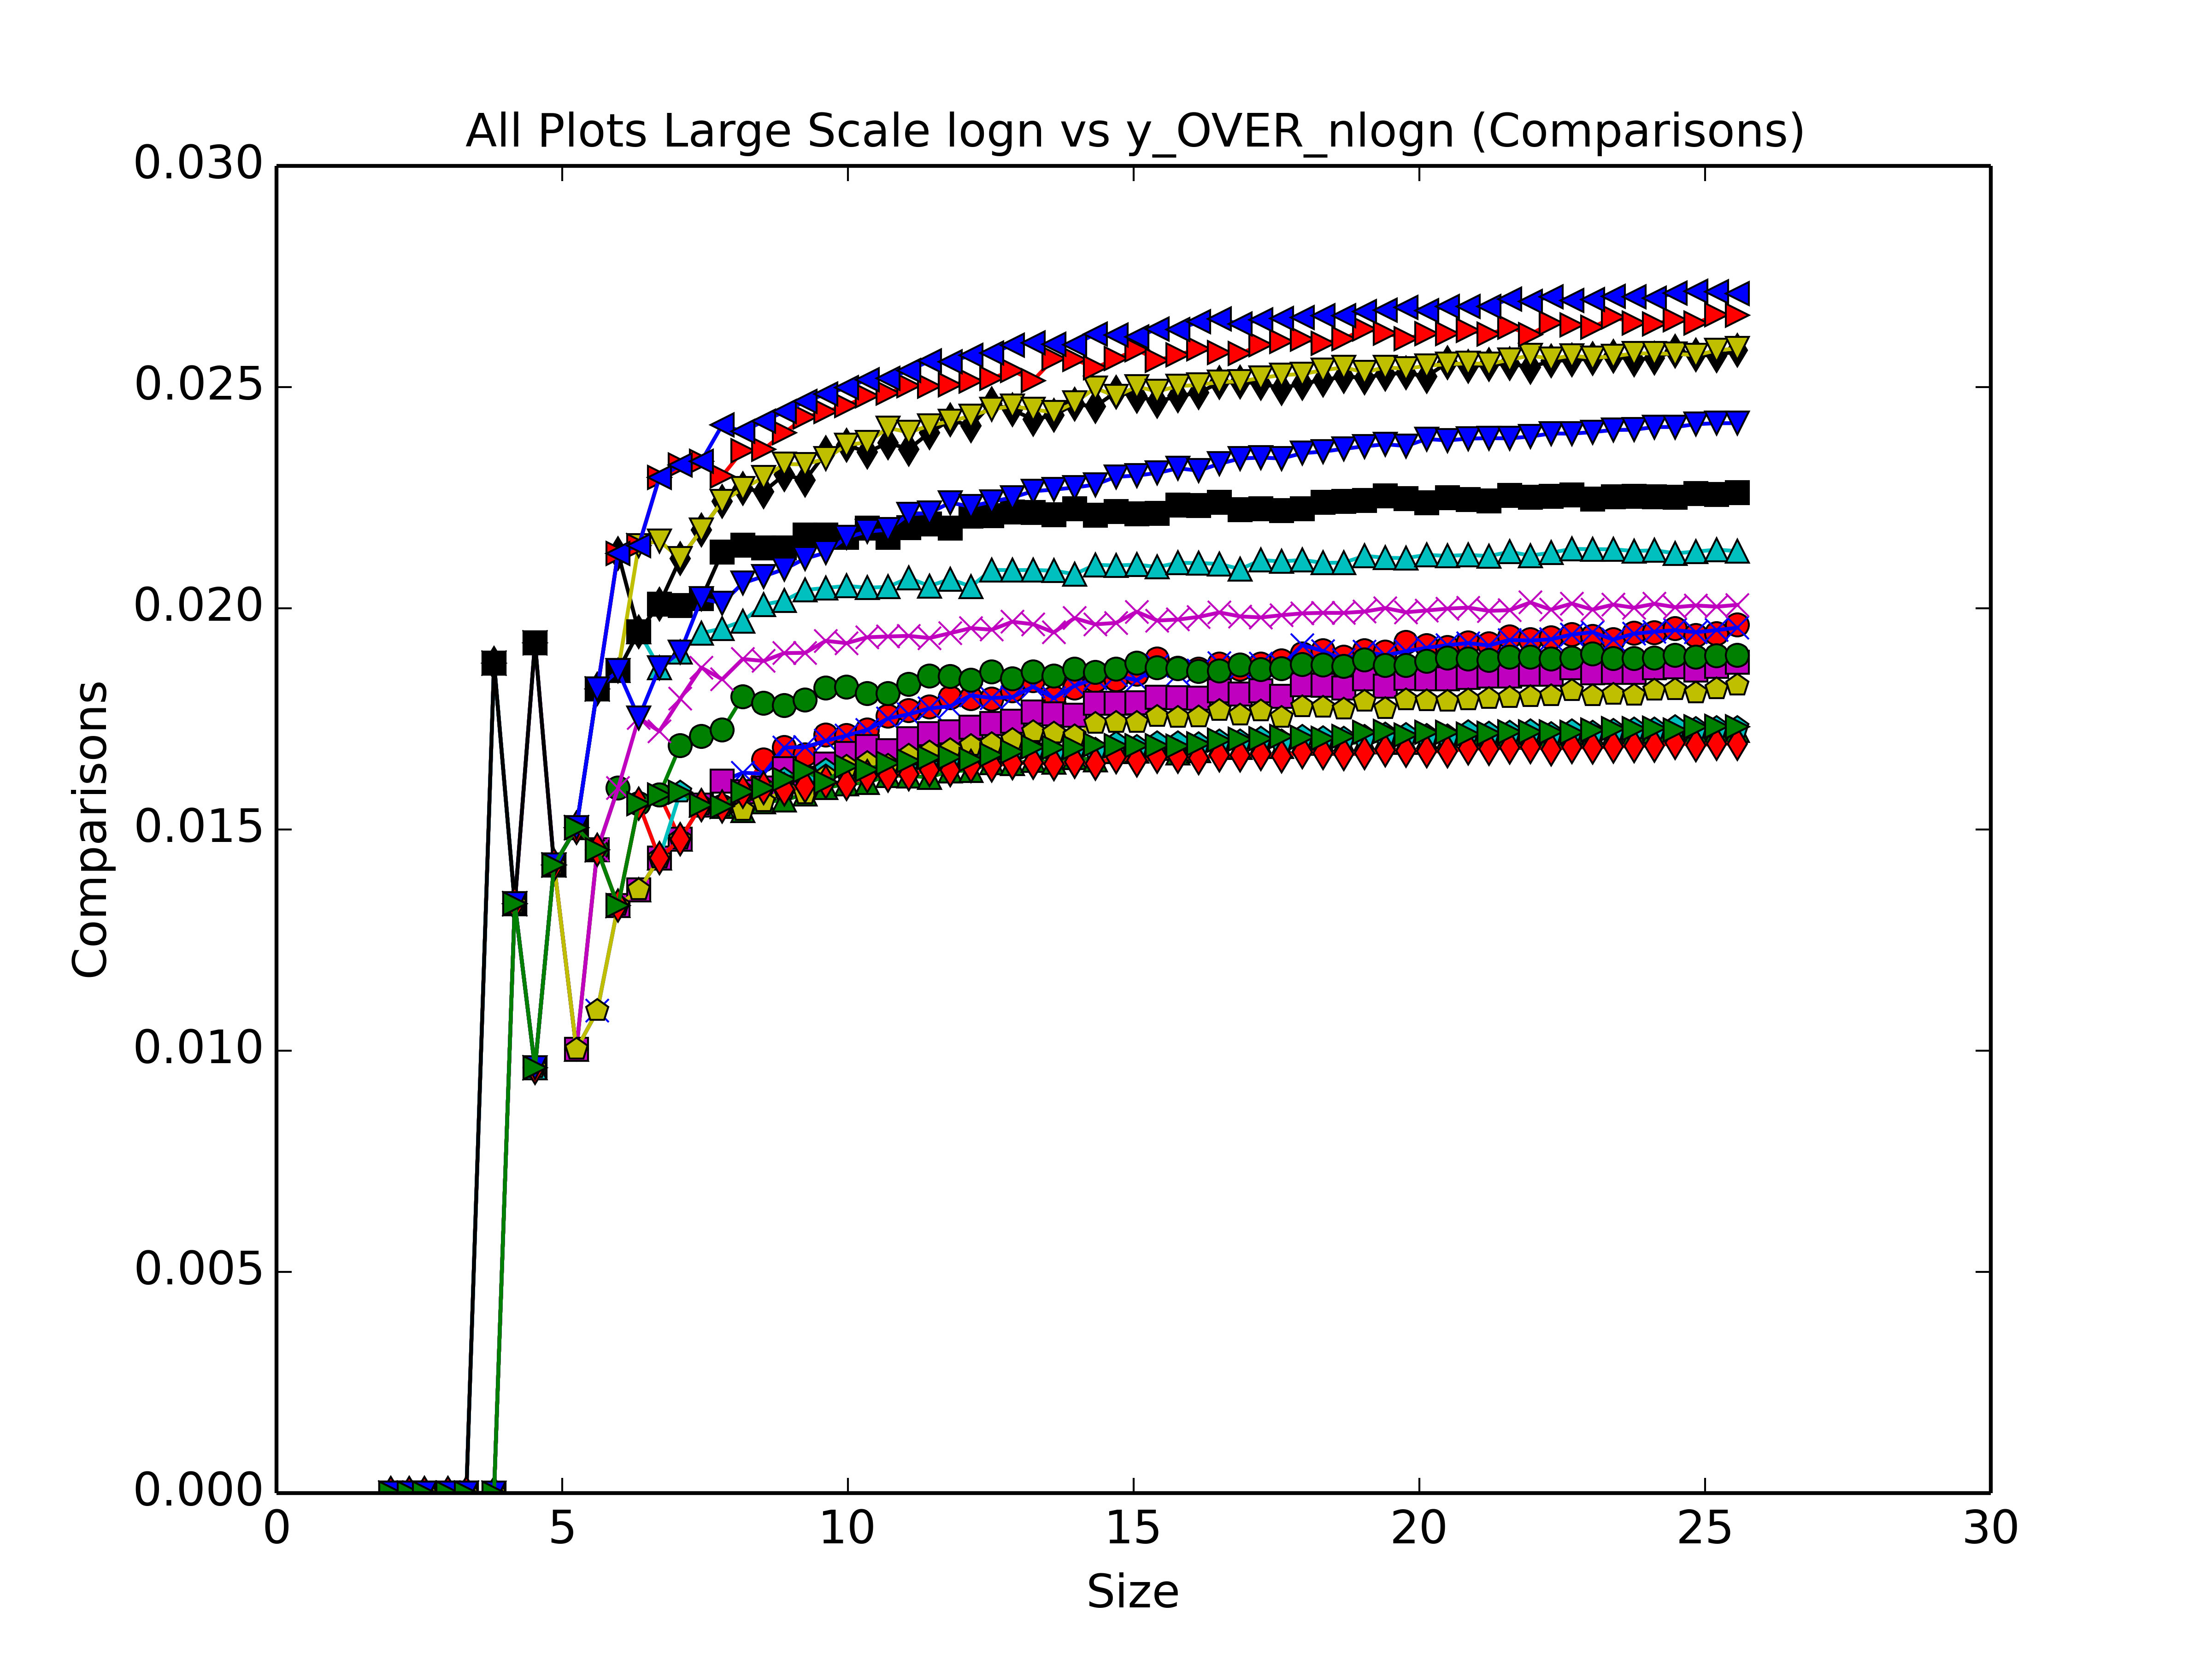
\includegraphics[width=150mm]{AllPlotsLargeScalelognvsy_OVER_nlogn_comp.png}
				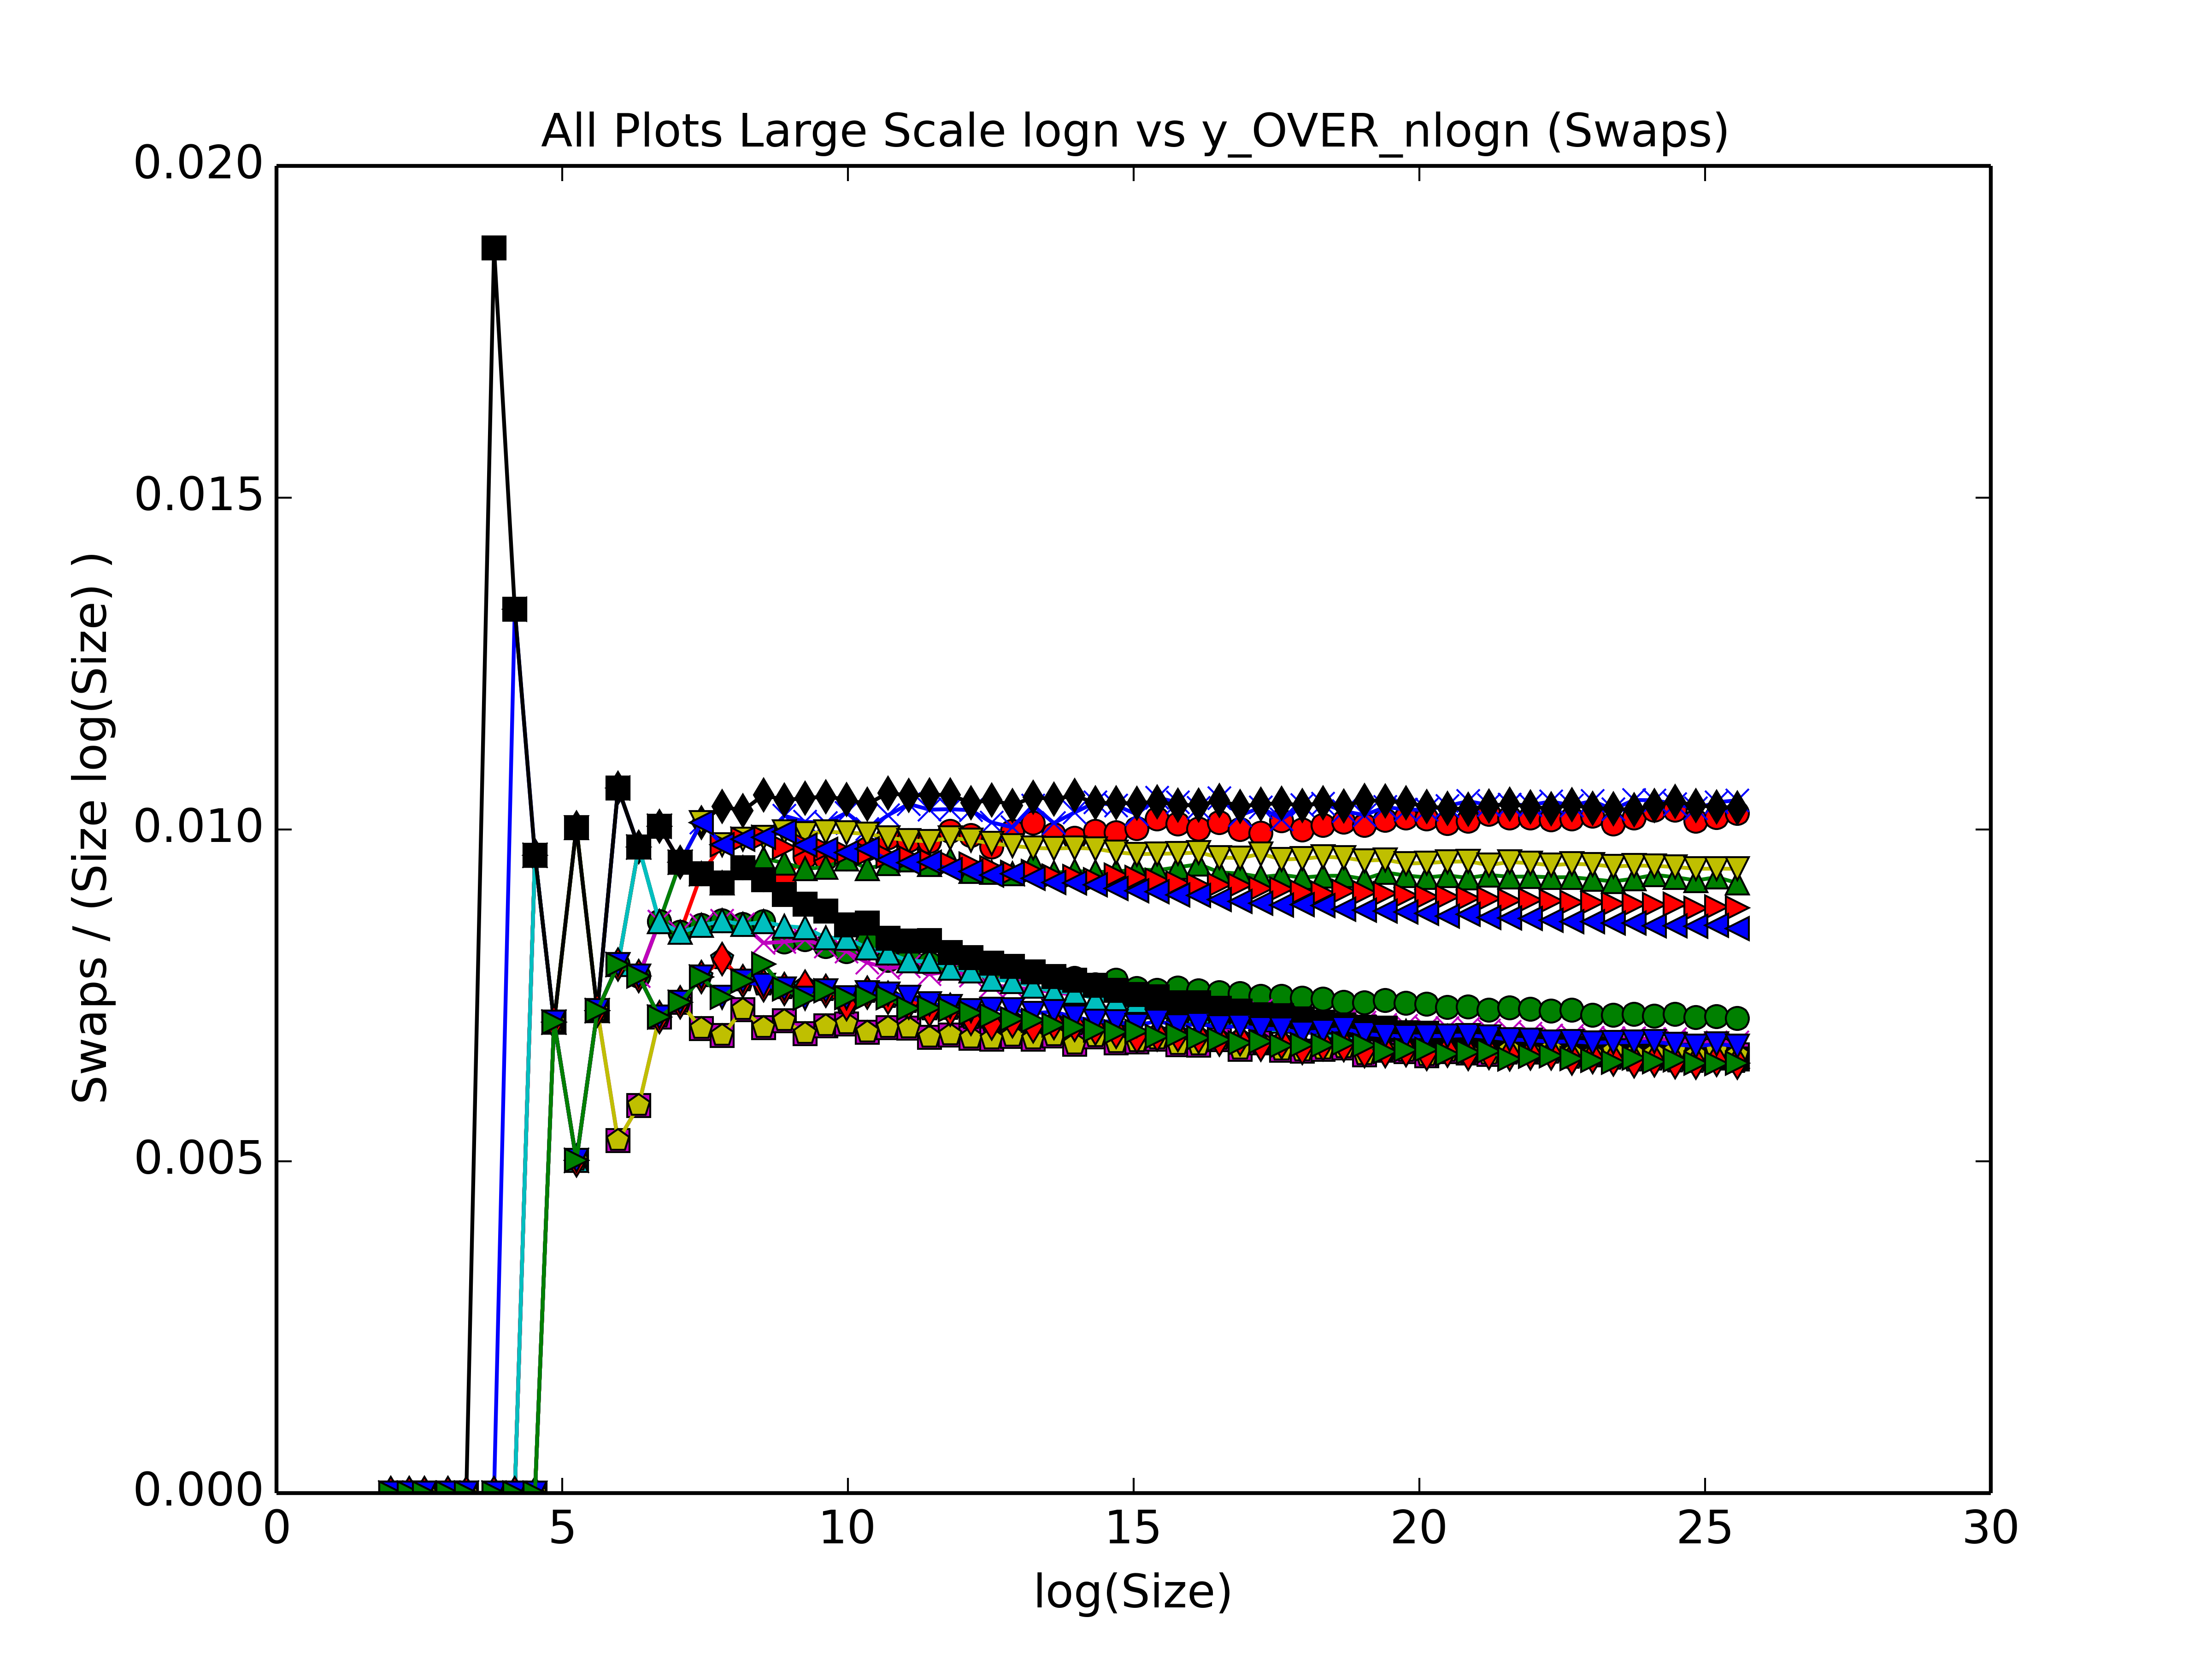
\includegraphics[width=150mm]{AllPlotsLargeScalelognvsy_OVER_nlogn_swap.png}
				\caption{A plot of the data from all the sorting algorithm}
				\label{fig:AllSortsLog}
			\end{center}
		\end{figure}

	\subsection{Non-Linear Curve Fit}
		\label{subsec:CurveFit}

		With the data that has collected we wish to be able to look at a whole data set and quantitatively compare
		to other data sets. From our introduction of the different quicksort algorithms,
		the asymptotic runtime of all of the had one of the following forms:
		\begin{equation}
			A\cdot n\log(n) + B\cdot n + \BigOh{\log(n)}
		\end{equation}
		\begin{equation}
			A\cdot n\log(n) + \BigOh{n}
		\end{equation}
		\begin{equation}
			\BigOh{n\log(n)}
		\end{equation}
		In correspondence of this we will fit the data to the following equation:
		\begin{equation}
			A\cdot n\log(n) + B\cdot n + C\log(n)
		\end{equation}
		With the function parameters $A,B$ and $C$ where found using a non-linear curve fitting tool in the SciPy module in python.
		Qualitatively, the fit function that was picked seems to result in good fits visually.
		Though the fit has less meaning do to the fact we don't have error bars on the data.
		A closer look at the reduced chi squared values of the fits leads us to believe that the fits are not good.\cite{bevington1969data}
		Thus we will treat the results from the best fit as qualitative.
		

\section{Discussion}
	\label{sec:Discussion}
	\subsection{$n\log(n)$ Trend}
		% Talk about \ref{fig:AllSortsLog}
		% This plot shows that the data is tapering off to a constant
		% But if you look at the axis, this is confirming the n log n
		% Behavior of the data and the algorithms

		% Talk about the plots and how each sort algorithm does relative to the others.
		Preliminary observations on Figure \ref{fig:AllSorts} show that the optimal dual pivot quicksort had the lowest number of comparisons.
		This is as expected since it was designed to minimize the number of comparisons.

	\subsection{Comparisons among Quicksorts}
		%Large Scale mass data
		%Comparisons :
		%	Optimized dual pivot quicksort, yaro, M-pivot sorts do well
		%	Heap Optimized m-pivot sorts do badly
		%Swaps :
		%	Heap Optimized Sorts still do badly relative to the rest.
		%	Classic quicksorts also doing badly.

		% Two pivot plots
		%Comparisons :
		%	We can start to see them split.
		%	Optimal Dual Pivot Quicksort [second option] still rocks.
		%	Dual Picot [1] and Optimal Dual Pivot [1] don't do well.
		%Swaps :
		%	They all do very similarly.
		%	Optimal Dual [1] and Dual Pivot [1] start to split away.
		
		% Three pivot plots
		%Comparisons :
		%	Interpretations Clear From plot.
		%	3-Pivot Sort is great then the Three-pivot-Quicksort
		%Swaps :
		%	Three-pivot-Quicksort is great then the 3-Pivot Sort
		%
		%In both cases heap 3-pivot sort is the worst.


		% All the M-pivot plots even with heap optimization
		%Comparisons :
		%	3,4,5-pivot sort are really good.
		%	All the heap-m-pivot sorts are not
		%Swaps :
		%	6-pivot sort is the best.
		%	Although 3,4,5-pivot sorts are good as well.
		%	All the heap-m-pivot sorts are not good.

		%**********************************************************************
		% Qualitatively compare them with there fit coefficients
		%**********************************************************************

	\subsection{Fit Functions}
		% Talk about the fit values, remember we are treating these values as qualitative
		% Talk about best and worst algorithms in terms of swaps and comparisons
		% Remember that the fit coefficients table has been updated.

		% Talk about the other functions that we have tried to fit

	\subsection{Future Work}
		\label{subsec:FutureStuff}
		% Talk about looking for more sorts
		% Talk about other distributions for random numbers
		% Talk about applying on nearly sorted arrays.
		% Talk about trying to measure time
		Read the comments in the .tex file

\section{Conclusion}
	\label{sec:Conclusionn}
	We did things and stuff!



%**********************************************************************
% Place the following in the appendix
%**********************************************************************

\section{Fit Coefficients}
	\label{sec:FitCoefficients}

	% (name,medianSelection,numPivots,usedInsertionSort)
	%***************************************************************************************************
	% FIT PARAMETERS FOR COMPARISONS
	%***************************************************************************************************
	\begin{table}
		\begin{center}
			\begin{tabular}{|r|c|c|c}
				\hline
								Sort Method              &   $A_{\text{comparisons}}$      \\ \hline \hline
				                Classic Quicksort - 1 - 1 &   $0.02151 \pm  0.00019$ \\ \hline
				                Classic Quicksort - 2 - 1 &   $0.02135 \pm  0.00017$ \\ \hline
				                Classic Quicksort - 3 - 1 &   $0.01807 \pm  0.00006$ \\ \hline
				              DualPivot Quicksort - 1 - 2 &   $0.02014 \pm  0.00018$ \\ \hline
				              DualPivot Quicksort - 2 - 2 &   $0.01772 \pm  0.00007$ \\ \hline
				 Heap Optimized M-Pivot Quicksort - 1 - 3 &   $0.02778 \pm  0.00014$ \\ \hline
				 Heap Optimized M-Pivot Quicksort - 1 - 4 &   $0.02788 \pm  0.00015$ \\ \hline
				 Heap Optimized M-Pivot Quicksort - 1 - 5 &   $0.02842 \pm  0.00025$ \\ \hline
				 Heap Optimized M-Pivot Quicksort - 1 - 6 &   $0.02869 \pm  0.00011$ \\ \hline
				                M-Pivot Quicksort - 1 - 3 &   $0.01970 \pm  0.00009$ \\ \hline
				                M-Pivot Quicksort - 1 - 4 &   $0.02076 \pm  0.00015$ \\ \hline
				                M-Pivot Quicksort - 1 - 5 &   $0.02165 \pm  0.00010$ \\ \hline
				                M-Pivot Quicksort - 1 - 6 &   $0.02386 \pm  0.00014$ \\ \hline
				     Optimal Dual Pivot Quicksort - 1 - 2 &   $0.01959 \pm  0.00019$ \\ \hline
				     Optimal Dual Pivot Quicksort - 2 - 2 &   $0.01744 \pm  0.00007$ \\ \hline
				            Three Pivot Quicksort - 1 - 3 &   $0.02587 \pm  0.00009$ \\ \hline
				           Yaroslavskiy Quicksort - 1 - 2 &   $0.01796 \pm  0.00010$ \\ \hline
			\end{tabular}
			\caption{Summary table coefficients of the non-linear fit for the parameter $A$ on the comparison data.}
			\label{tab:compFitCoeffA}
		\end{center}
	\end{table}


	\begin{table}
		\begin{center}
			\begin{tabular}{|r|c|c|c}
				\hline
								Sort Method              &   $B_{\text{comparisons}}$      \\ \hline \hline
				                Classic Quicksort - 1 - 1 &   $-0.05025 \pm  0.00469$ \\ \hline
				                Classic Quicksort - 2 - 1 &   $-0.04634 \pm  0.00428$ \\ \hline
				                Classic Quicksort - 3 - 1 &   $-0.02126 \pm  0.00163$ \\ \hline
				              DualPivot Quicksort - 1 - 2 &   $-0.03650 \pm  0.00465$ \\ \hline
				              DualPivot Quicksort - 2 - 2 &   $-0.01045 \pm  0.00183$ \\ \hline
				 Heap Optimized M-Pivot Quicksort - 1 - 3 &   $-0.05055 \pm  0.00355$ \\ \hline
				 Heap Optimized M-Pivot Quicksort - 1 - 4 &   $-0.05152 \pm  0.00368$ \\ \hline
				 Heap Optimized M-Pivot Quicksort - 1 - 5 &   $-0.04639 \pm  0.00626$ \\ \hline
				 Heap Optimized M-Pivot Quicksort - 1 - 6 &   $-0.03889 \pm  0.00280$ \\ \hline
				                M-Pivot Quicksort - 1 - 3 &   $-0.01917 \pm  0.00220$ \\ \hline
				                M-Pivot Quicksort - 1 - 4 &   $-0.01716 \pm  0.00391$ \\ \hline
				                M-Pivot Quicksort - 1 - 5 &   $-0.00902 \pm  0.00244$ \\ \hline
				                M-Pivot Quicksort - 1 - 6 &   $-0.03206 \pm  0.00366$ \\ \hline
				     Optimal Dual Pivot Quicksort - 1 - 2 &   $-0.03580 \pm  0.00490$ \\ \hline
				     Optimal Dual Pivot Quicksort - 2 - 2 &   $-0.01266 \pm  0.00165$ \\ \hline
				            Three Pivot Quicksort - 1 - 3 &   $-0.04282 \pm  0.00232$ \\ \hline
				           Yaroslavskiy Quicksort - 1 - 2 &   $-0.01636 \pm  0.00251$ \\ \hline
			\end{tabular}
			\caption{Summary table coefficients of the non-linear fit for the parameter $B$ on the comparison data.}
			\label{tab:compFitCoeffB}
		\end{center}
	\end{table}

	\begin{table}
		\begin{center}
			\begin{tabular}{|r|c|c|c}
				\hline
								Sort Method              &   $C_{\text{comparisons}}$      \\ \hline \hline
				                Classic Quicksort - 1 - 1 &  $ 121.34341 \pm  99.97322$ \\ \hline
				                Classic Quicksort - 2 - 1 &  $  78.33233 \pm  91.31275$ \\ \hline
				                Classic Quicksort - 3 - 1 &  $  22.52742 \pm  34.75034$ \\ \hline
				              DualPivot Quicksort - 1 - 2 &  $  52.22569 \pm  99.17037$ \\ \hline
				              DualPivot Quicksort - 2 - 2 &  $ -53.25104 \pm  39.07336$ \\ \hline
				 Heap Optimized M-Pivot Quicksort - 1 - 3 &  $  94.09226 \pm  75.71998$ \\ \hline
				 Heap Optimized M-Pivot Quicksort - 1 - 4 &  $ 124.92512 \pm  78.46872$ \\ \hline
				 Heap Optimized M-Pivot Quicksort - 1 - 5 &  $  56.97527 \pm 133.52044$ \\ \hline
				 Heap Optimized M-Pivot Quicksort - 1 - 6 &  $  29.84293 \pm  59.67899$ \\ \hline
				                M-Pivot Quicksort - 1 - 3 &  $  51.60730 \pm  46.87649$ \\ \hline
				                M-Pivot Quicksort - 1 - 4 &  $  49.35746 \pm  83.31083$ \\ \hline
				                M-Pivot Quicksort - 1 - 5 &  $   4.76647 \pm  52.03322$ \\ \hline
				                M-Pivot Quicksort - 1 - 6 &  $ 136.38815 \pm  77.96382$ \\ \hline
				     Optimal Dual Pivot Quicksort - 1 - 2 &  $  56.95127 \pm 104.39452$ \\ \hline
				     Optimal Dual Pivot Quicksort - 2 - 2 &  $ -26.20004 \pm  35.22097$ \\ \hline
				            Three Pivot Quicksort - 1 - 3 &  $ -17.79746 \pm  49.38183$ \\ \hline
				           Yaroslavskiy Quicksort - 1 - 2 &  $   0.73204 \pm  53.59187$ \\ \hline
			\end{tabular}
			\caption{Summary table coefficients of the non-linear fit for the parameter $C$ on the comparison data.}
			\label{tab:compFitCoeffC}
		\end{center}
	\end{table}



	%***************************************************************************************************
	% FIT PARAMETERS FOR SWAPS
	%***************************************************************************************************



	\begin{table}
		\begin{center}
			\begin{tabular}{|r|c|c|c}
				\hline
								Sort Method              &   $A_{\text{swap}}$      \\ \hline \hline
				                Classic Quicksort - 1 - 1 &   $0.01026 \pm  0.00017$ \\ \hline
				                Classic Quicksort - 2 - 1 &   $0.01095 \pm  0.00016$ \\ \hline
				                Classic Quicksort - 3 - 1 &   $0.00848 \pm  0.00012$ \\ \hline
				              DualPivot Quicksort - 1 - 2 &   $0.00629 \pm  0.00010$ \\ \hline
				              DualPivot Quicksort - 2 - 2 &   $0.00606 \pm  0.00006$ \\ \hline
				 Heap Optimized M-Pivot Quicksort - 1 - 3 &   $0.01004 \pm  0.00009$ \\ \hline
				 Heap Optimized M-Pivot Quicksort - 1 - 4 &   $0.00898 \pm  0.00004$ \\ \hline
				 Heap Optimized M-Pivot Quicksort - 1 - 5 &   $0.00809 \pm  0.00004$ \\ \hline
				 Heap Optimized M-Pivot Quicksort - 1 - 6 &   $0.00759 \pm  0.00005$ \\ \hline
				                M-Pivot Quicksort - 1 - 3 &   $0.00672 \pm  0.00006$ \\ \hline
				                M-Pivot Quicksort - 1 - 4 &   $0.00605 \pm  0.00003$ \\ \hline
				                M-Pivot Quicksort - 1 - 5 &   $0.00535 \pm  0.00003$ \\ \hline
				                M-Pivot Quicksort - 1 - 6 &   $0.00513 \pm  0.00003$ \\ \hline
				     Optimal Dual Pivot Quicksort - 1 - 2 &   $0.00629 \pm  0.00010$ \\ \hline
				     Optimal Dual Pivot Quicksort - 2 - 2 &   $0.00606 \pm  0.00006$ \\ \hline
				            Three Pivot Quicksort - 1 - 3 &   $0.00635 \pm  0.00006$ \\ \hline
				           Yaroslavskiy Quicksort - 1 - 2 &   $0.00586 \pm  0.00005$ \\ \hline
			\end{tabular}
			\caption{Summary table coefficients of the non-linear fit for the parameter $A$ on the swap data.}
			\label{tab:swapFitCoeffA}
		\end{center}
	\end{table}


	\begin{table}
		\begin{center}
			\begin{tabular}{|r|c|c|c}
				\hline
								Sort Method              &   $B_{\text{swap}}$      \\ \hline \hline
				                Classic Quicksort - 1 - 1 &   $ -0.00132 \pm  0.00442$ \\ \hline
				                Classic Quicksort - 2 - 1 &   $ -0.01411 \pm  0.00417$ \\ \hline
				                Classic Quicksort - 3 - 1 &   $  0.01903 \pm  0.00298$ \\ \hline
				              DualPivot Quicksort - 1 - 2 &   $  0.00824 \pm  0.00264$ \\ \hline
				              DualPivot Quicksort - 2 - 2 &   $  0.01080 \pm  0.00153$ \\ \hline
				 Heap Optimized M-Pivot Quicksort - 1 - 3 &   $  0.00774 \pm  0.00233$ \\ \hline
				 Heap Optimized M-Pivot Quicksort - 1 - 4 &   $  0.01111 \pm  0.00097$ \\ \hline
				 Heap Optimized M-Pivot Quicksort - 1 - 5 &   $  0.01881 \pm  0.00113$ \\ \hline
				 Heap Optimized M-Pivot Quicksort - 1 - 6 &   $  0.02363 \pm  0.00129$ \\ \hline
				                M-Pivot Quicksort - 1 - 3 &   $  0.01160 \pm  0.00156$ \\ \hline
				                M-Pivot Quicksort - 1 - 4 &   $  0.01890 \pm  0.00069$ \\ \hline
				                M-Pivot Quicksort - 1 - 5 &   $  0.03171 \pm  0.00065$ \\ \hline
				                M-Pivot Quicksort - 1 - 6 &   $  0.03601 \pm  0.00077$ \\ \hline
				     Optimal Dual Pivot Quicksort - 1 - 2 &   $  0.00824 \pm  0.00264$ \\ \hline
				     Optimal Dual Pivot Quicksort - 2 - 2 &   $  0.01080 \pm  0.00153$ \\ \hline
				            Three Pivot Quicksort - 1 - 3 &   $  0.01030 \pm  0.00153$ \\ \hline
				           Yaroslavskiy Quicksort - 1 - 2 &   $  0.01592 \pm  0.00127$ \\ \hline
			\end{tabular}
			\caption{Summary table coefficients of the non-linear fit for the parameter $B$ on the swap data.}
			\label{tab:swapFitCoeffB}
		\end{center}
	\end{table}

	\begin{table}
		\begin{center}
			\begin{tabular}{|r|c|c|c}
				\hline
								Sort Method              &   $C_{\text{swap}}$      \\ \hline \hline
				                Classic Quicksort - 1 - 1 &  $  -36.52075 \pm 94.28550 $ \\ \hline
				                Classic Quicksort - 2 - 1 &  $  102.34036 \pm 88.94077 $ \\ \hline
				                Classic Quicksort - 3 - 1 &  $ -103.21696 \pm 63.57056 $ \\ \hline
				              DualPivot Quicksort - 1 - 2 &  $  -38.02577 \pm 56.38166 $ \\ \hline
				              DualPivot Quicksort - 2 - 2 &  $   42.34411 \pm 32.52471 $ \\ \hline
				 Heap Optimized M-Pivot Quicksort - 1 - 3 &  $  -53.81114 \pm 49.78070 $ \\ \hline
				 Heap Optimized M-Pivot Quicksort - 1 - 4 &  $   -3.24127 \pm 20.75454 $ \\ \hline
				 Heap Optimized M-Pivot Quicksort - 1 - 5 &  $  -16.07787 \pm 24.00667 $ \\ \hline
				 Heap Optimized M-Pivot Quicksort - 1 - 6 &  $  -20.99394 \pm 27.47669 $ \\ \hline
				                M-Pivot Quicksort - 1 - 3 &  $   41.76450 \pm 33.26955 $ \\ \hline
				                M-Pivot Quicksort - 1 - 4 &  $   16.90493 \pm 14.70501 $ \\ \hline
				                M-Pivot Quicksort - 1 - 5 &  $  -17.36329 \pm 13.95680 $ \\ \hline
				                M-Pivot Quicksort - 1 - 6 &  $   -5.54593 \pm 16.46902 $ \\ \hline
				     Optimal Dual Pivot Quicksort - 1 - 2 &  $  -38.02577 \pm 56.38166 $ \\ \hline
				     Optimal Dual Pivot Quicksort - 2 - 2 &  $   42.34411 \pm 32.52471 $ \\ \hline
				            Three Pivot Quicksort - 1 - 3 &  $   14.68107 \pm 32.72260 $ \\ \hline
				           Yaroslavskiy Quicksort - 1 - 2 &  $    6.27071 \pm 27.13874 $ \\ \hline
			\end{tabular}
			\caption{Summary table coefficients of the non-linear fit for the parameter $C$ on the swap data.}
			\label{tab:swapFitCoeffC}
		\end{center}
	\end{table}


\section{Misc Plots}
	\label{sec:MiscPlots}

	%**********************************************************************
	% Dual Pivots Large Scale
	%**********************************************************************
	\begin{figure}[ht!]
		\begin{center}
			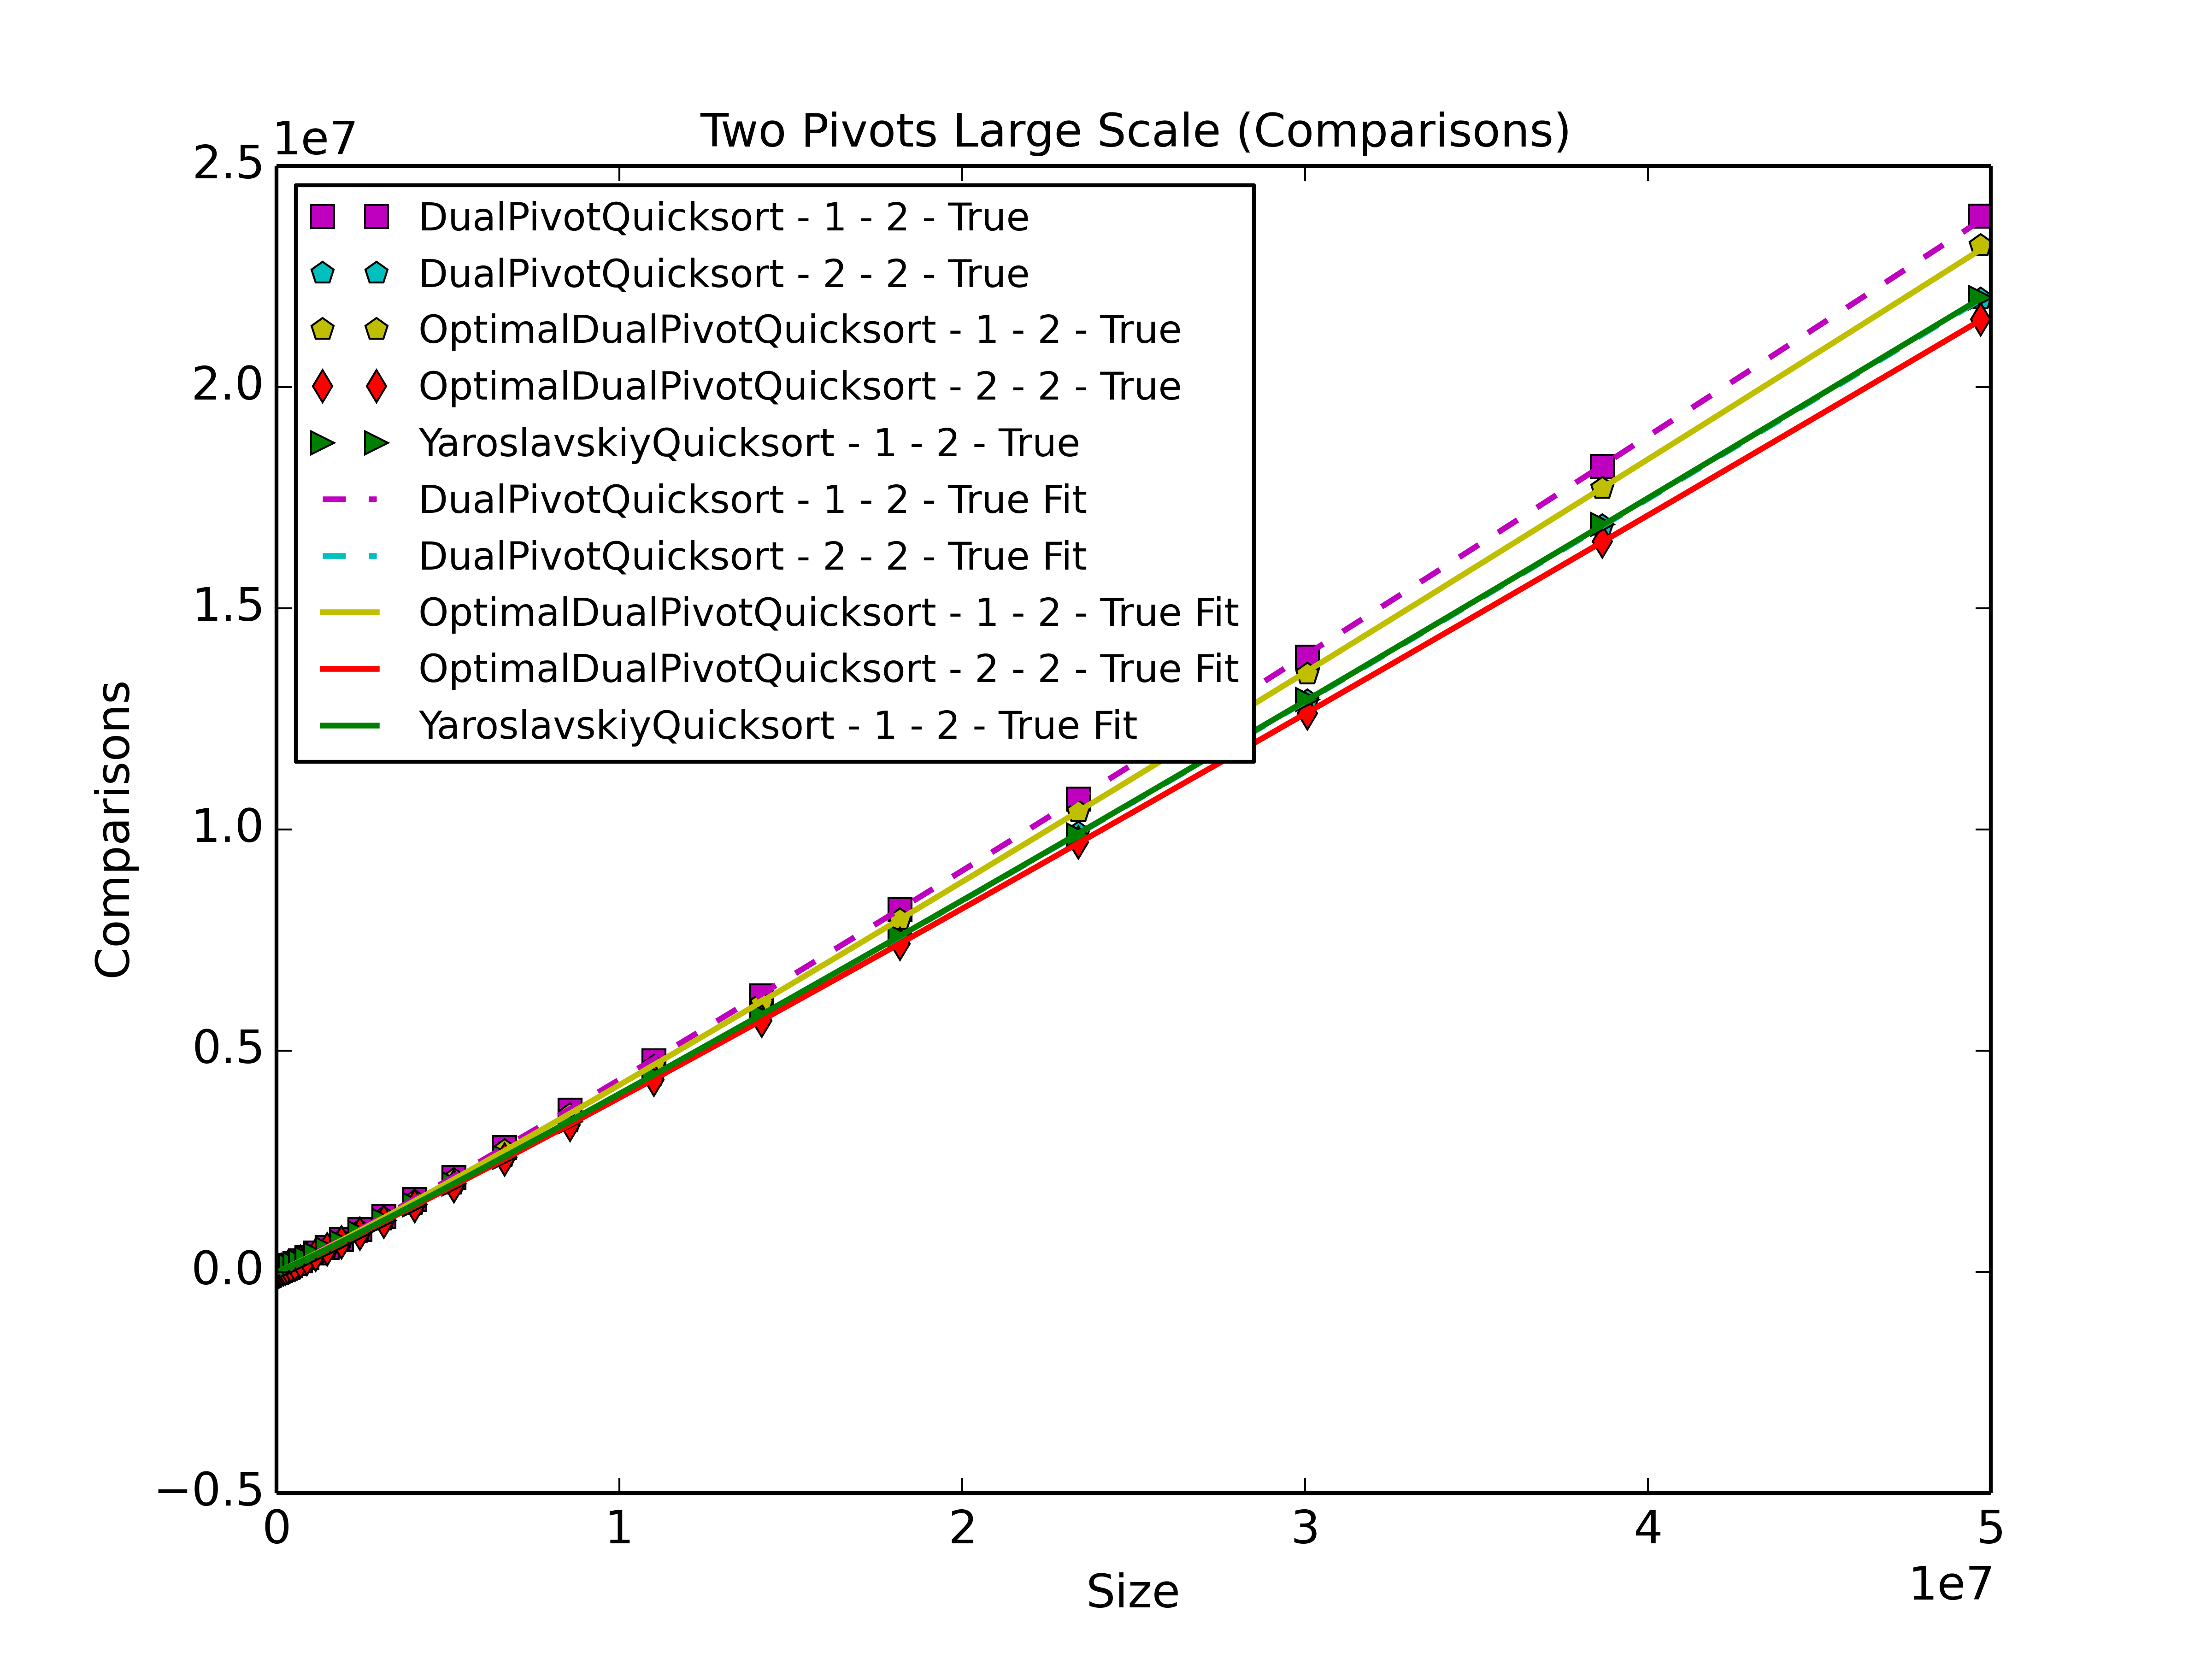
\includegraphics[width=150mm]{TwoPivotsLargeScale_comp.png}
			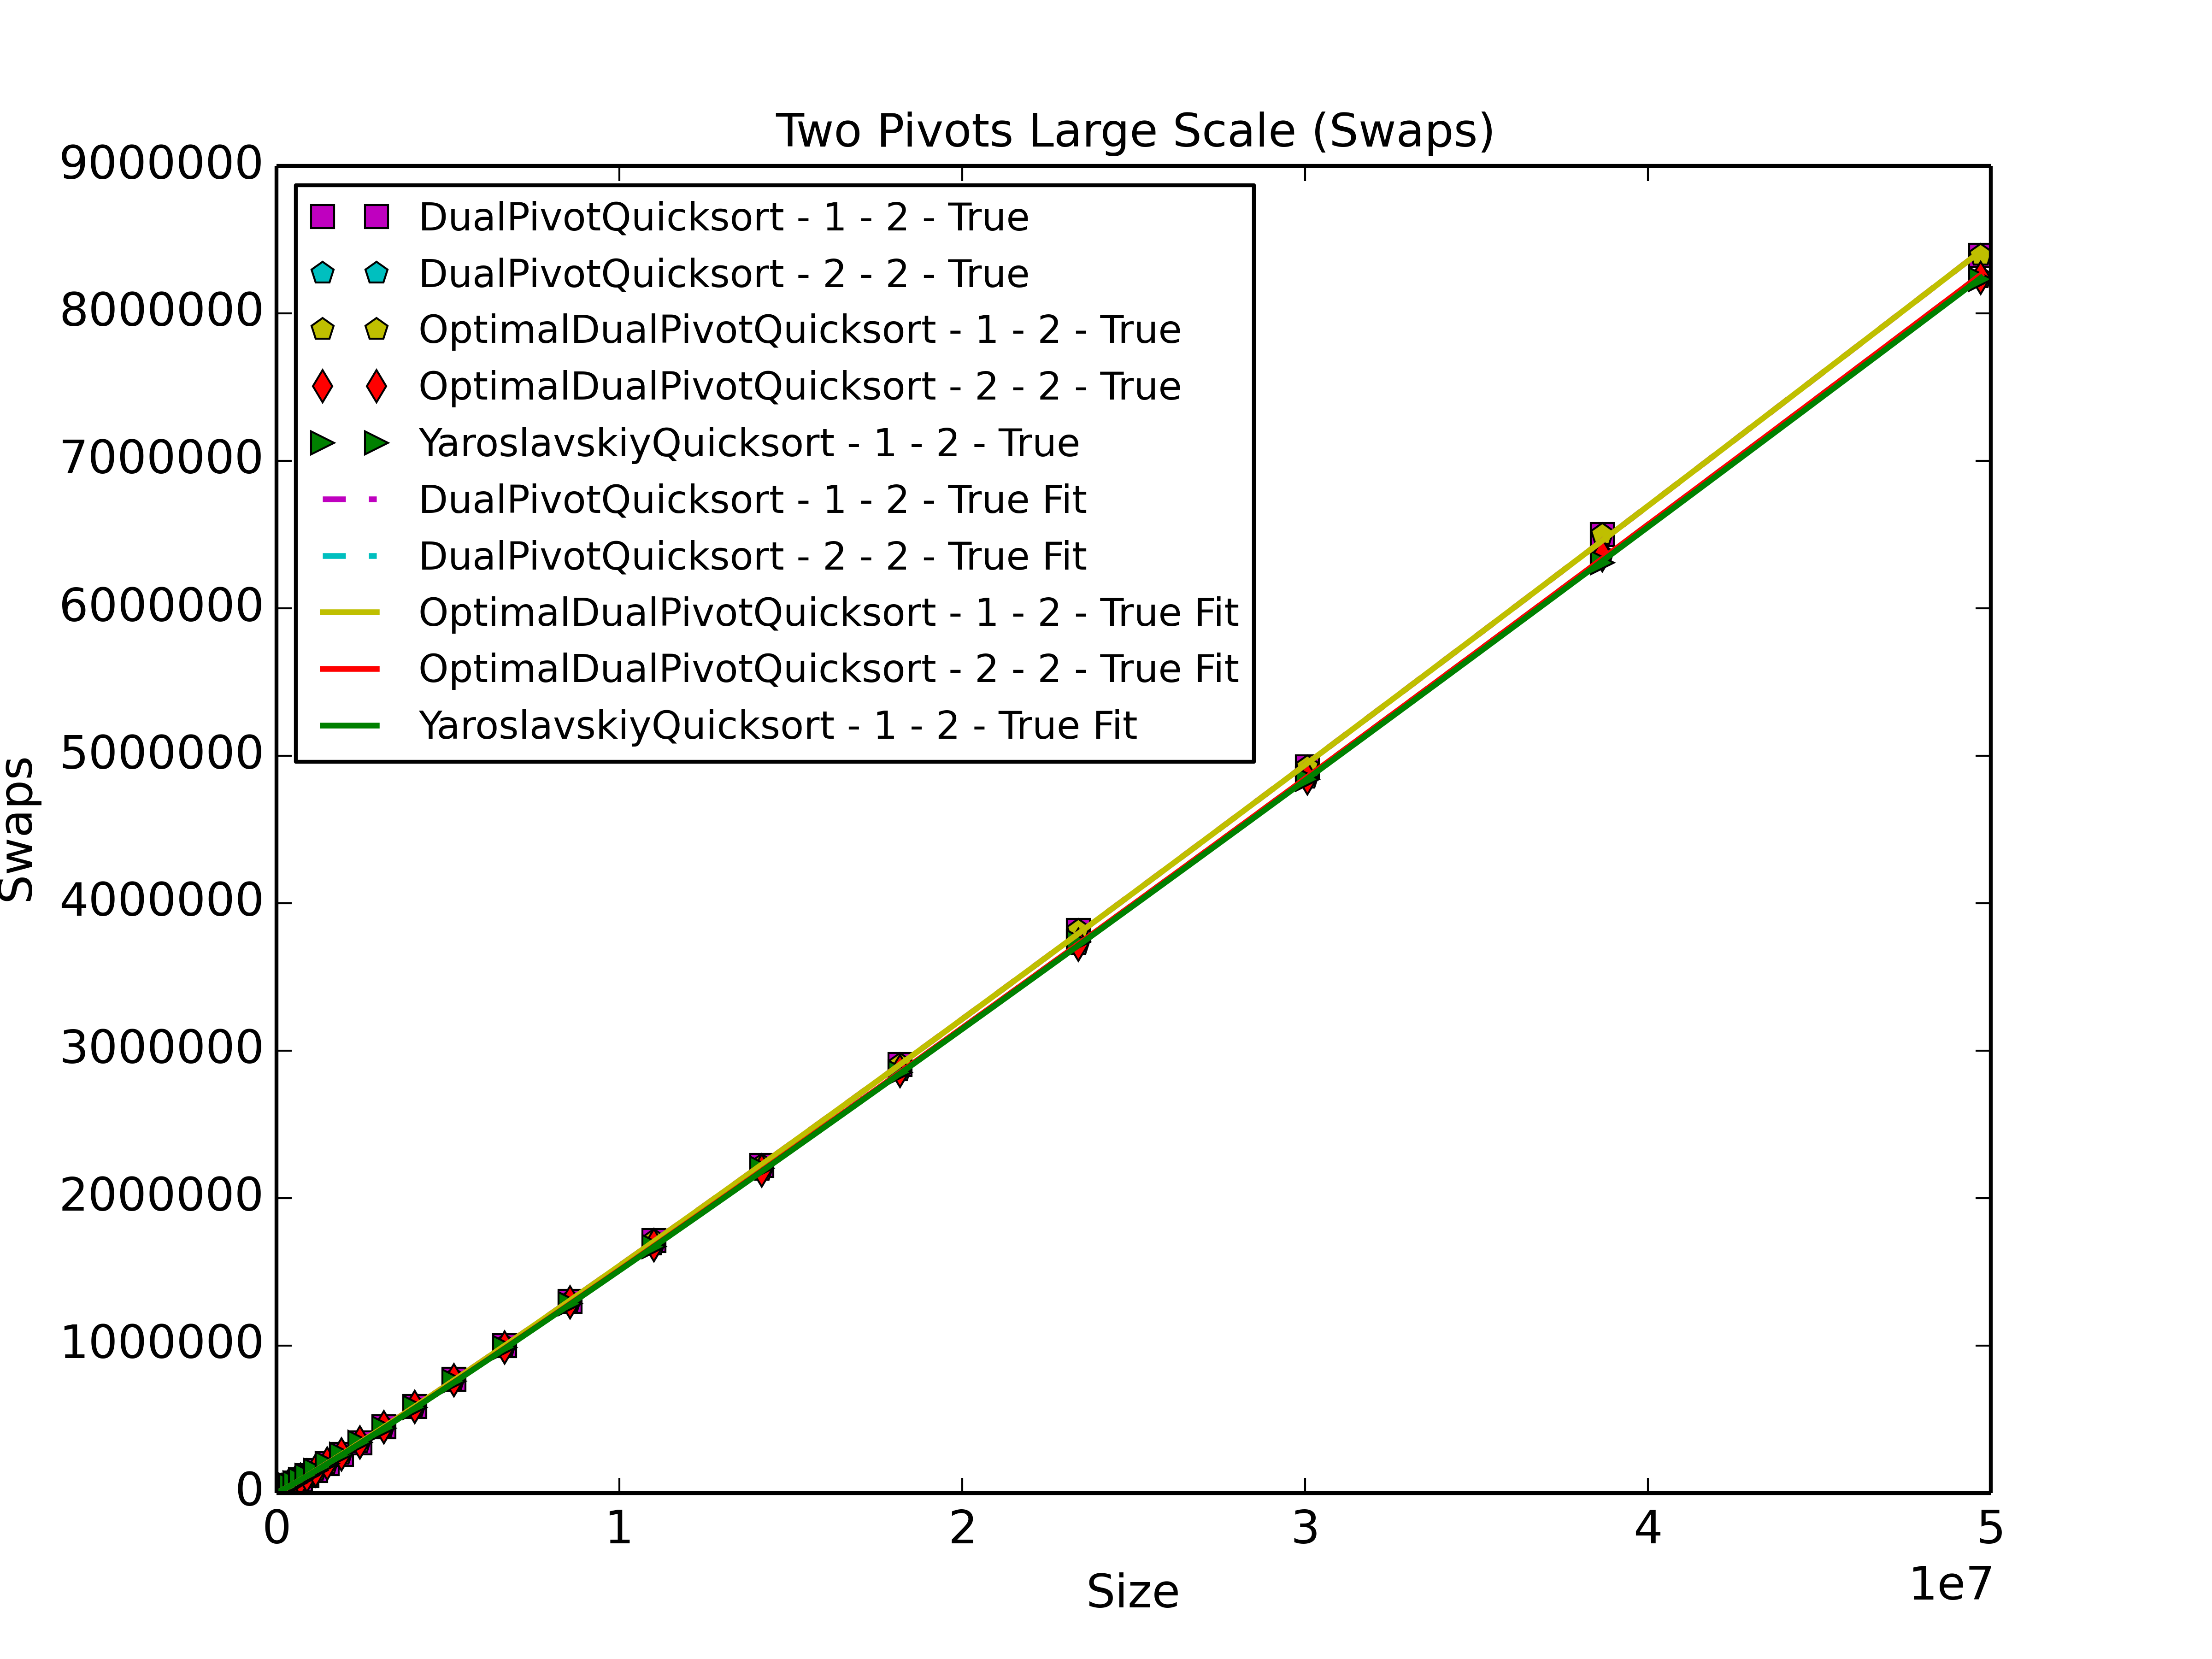
\includegraphics[width=150mm]{TwoPivotsLargeScale_swap.png}
			\caption{A plot of the data from all the sorting algorithm with two pivots}
		\label{fig:TwoPivot}
		\end{center}
	\end{figure}

	%**********************************************************************
	% Three Pivots Large Scale
	%**********************************************************************
	\begin{figure}[ht!]
		\begin{center}
			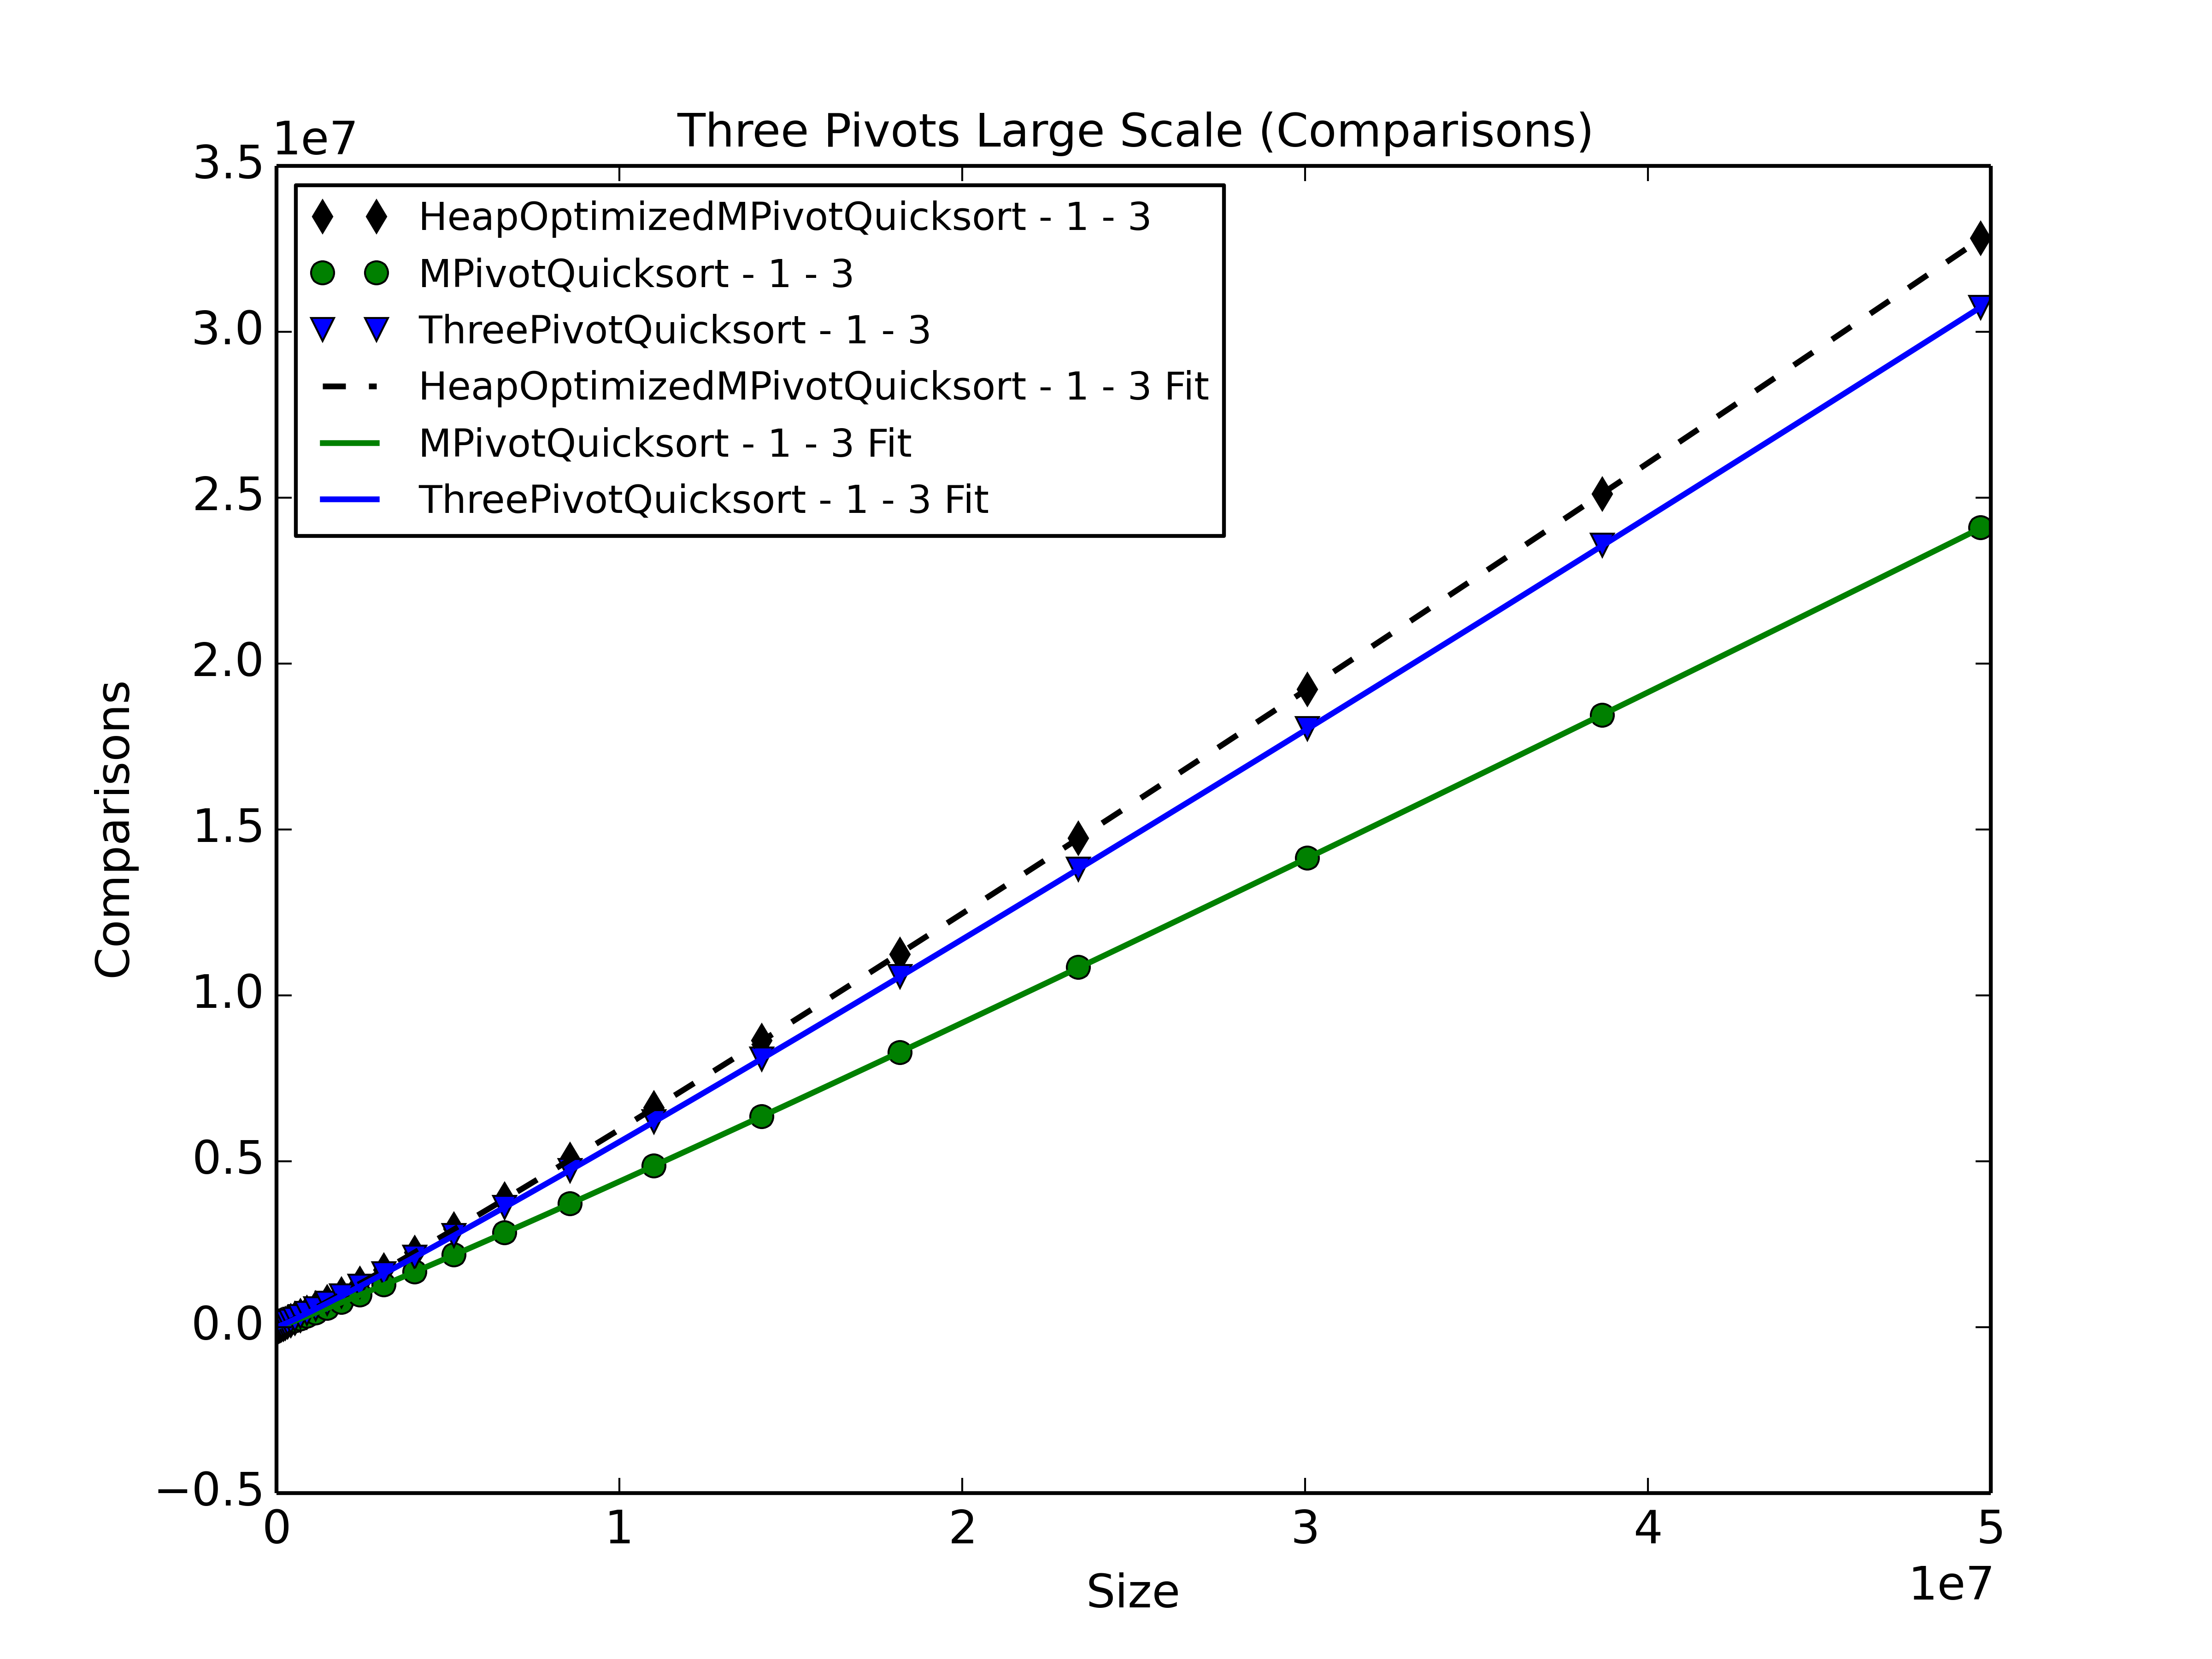
\includegraphics[width=150mm]{ThreePivotsLargeScale_comp.png}
			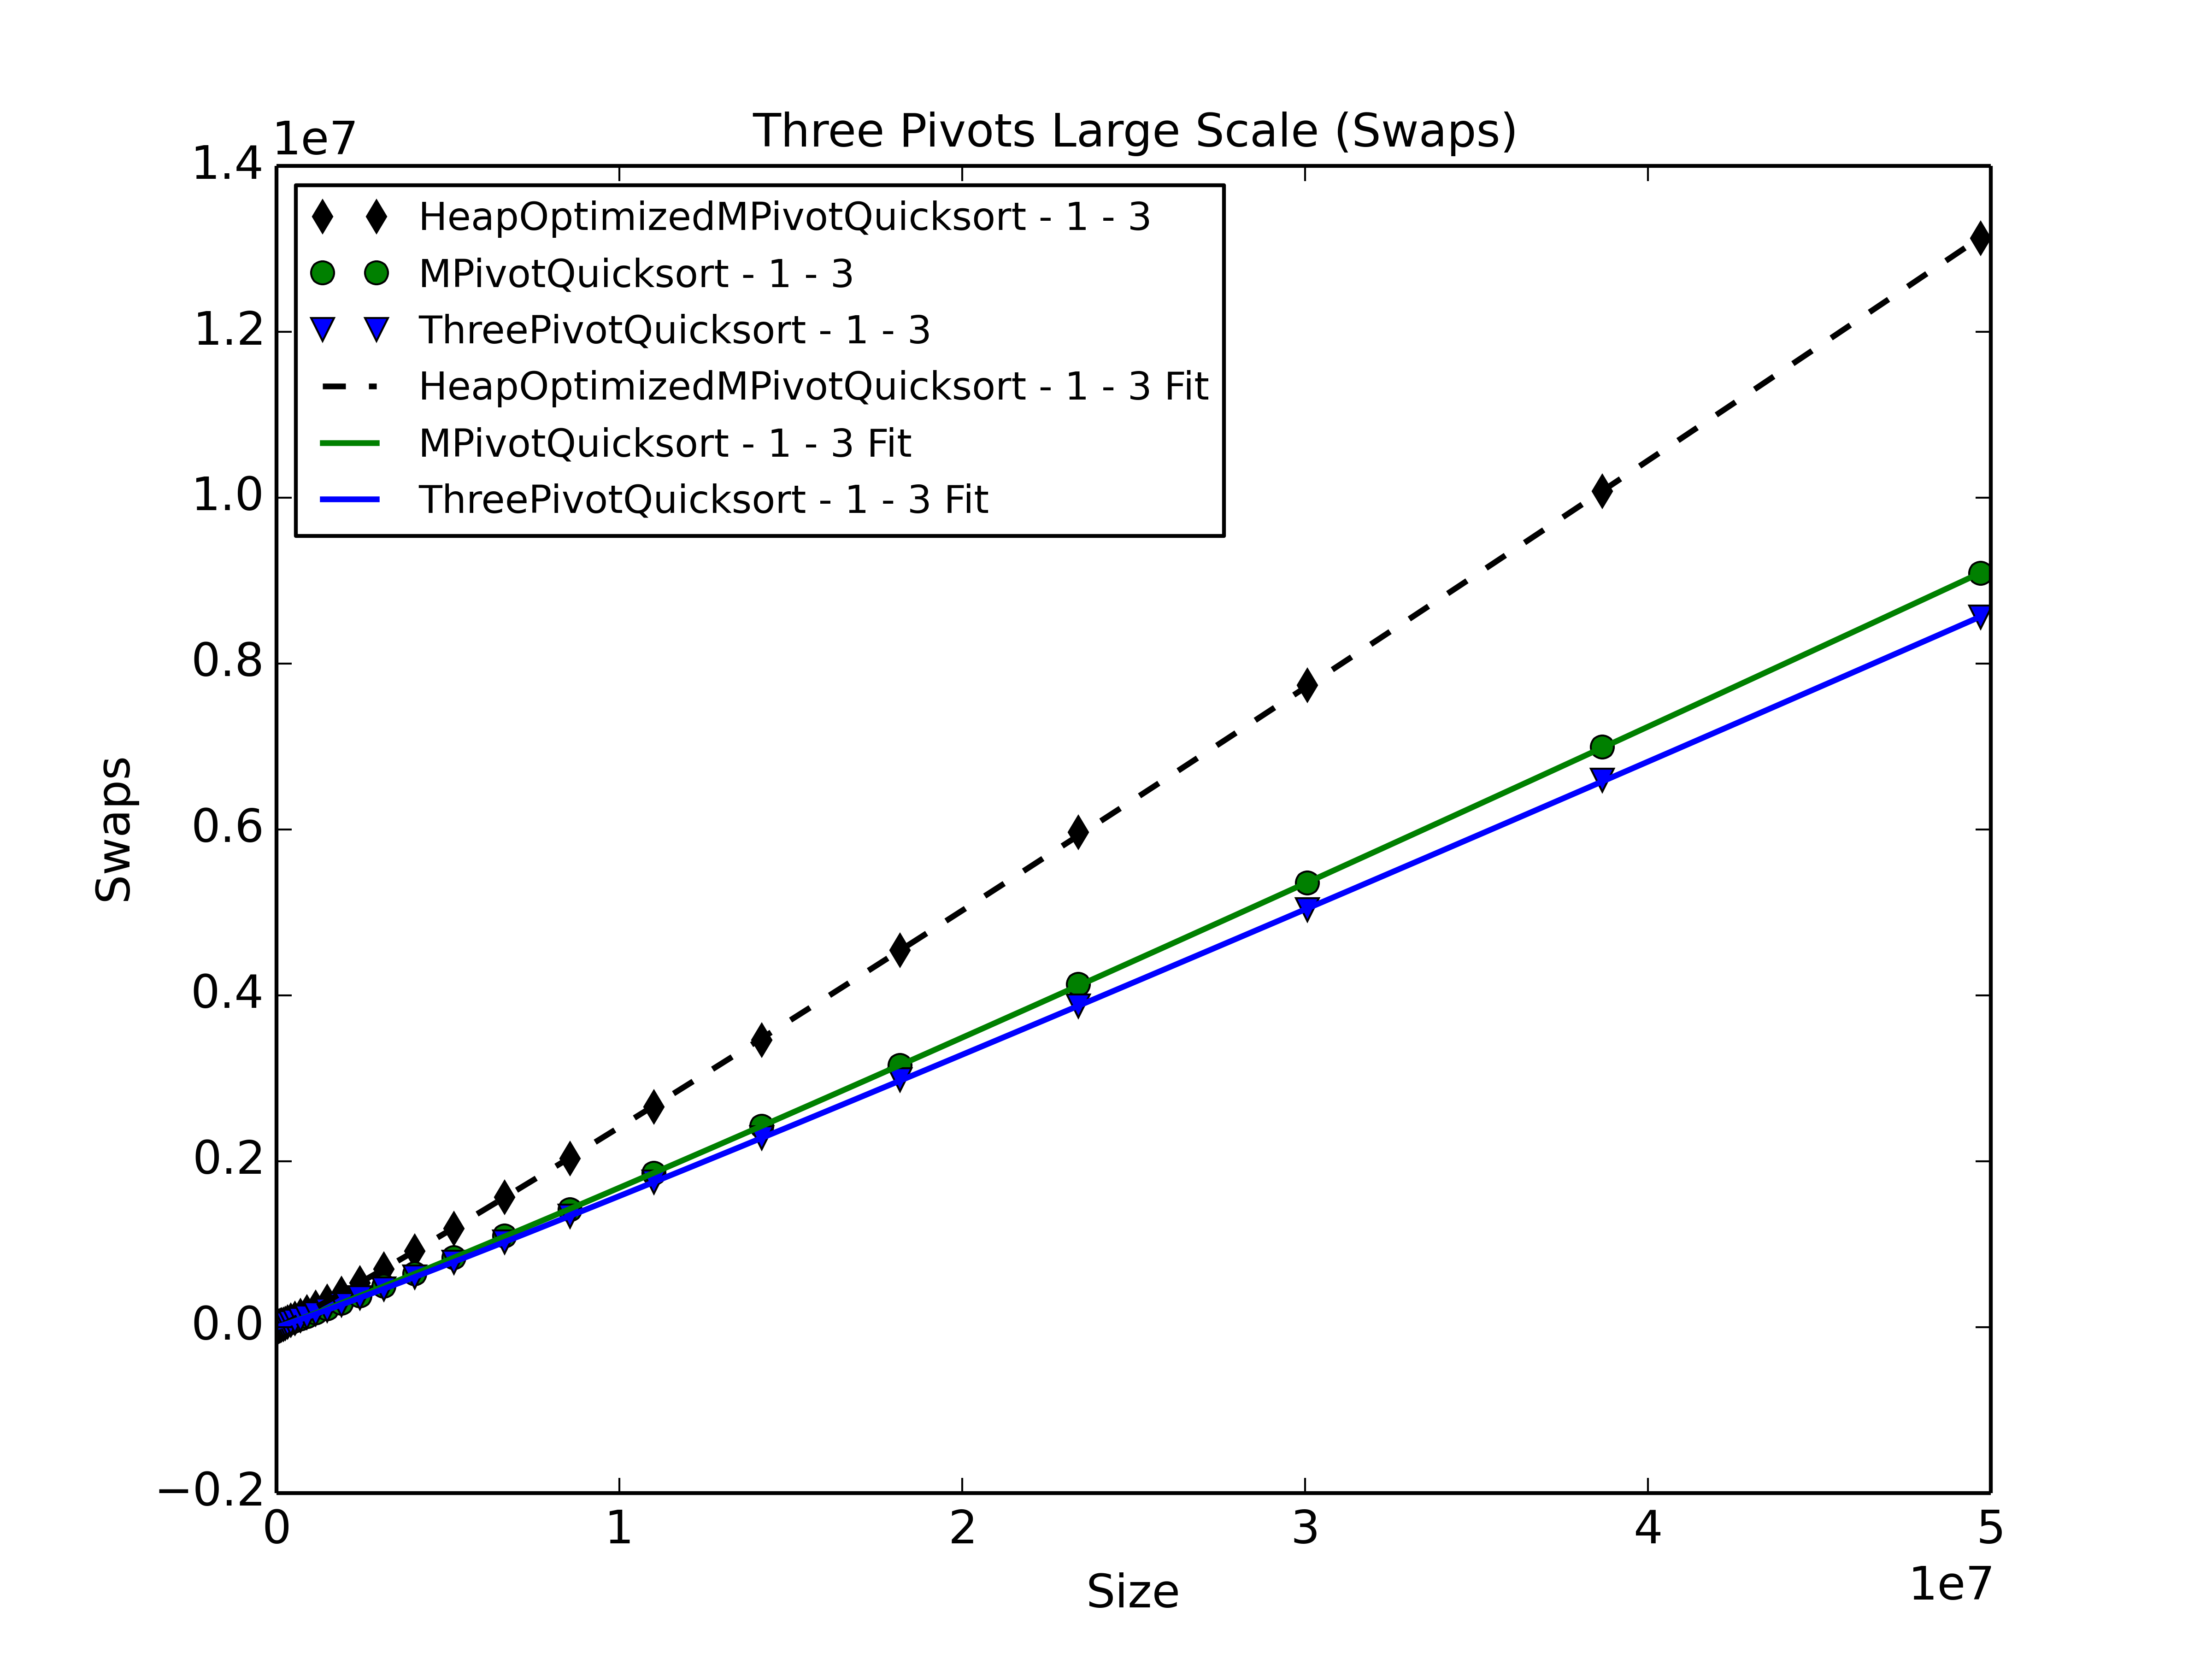
\includegraphics[width=150mm]{ThreePivotsLargeScale_swap.png}
			\caption{A plot of the data from all the sorting algorithm with three pivots}
			\label{fig:ThreePivot}
		\end{center}
	\end{figure}

	%**********************************************************************
	% M-Pivot Pivot Sorts Large Scale
	%**********************************************************************
	\begin{figure}[ht!]
		\begin{center}
			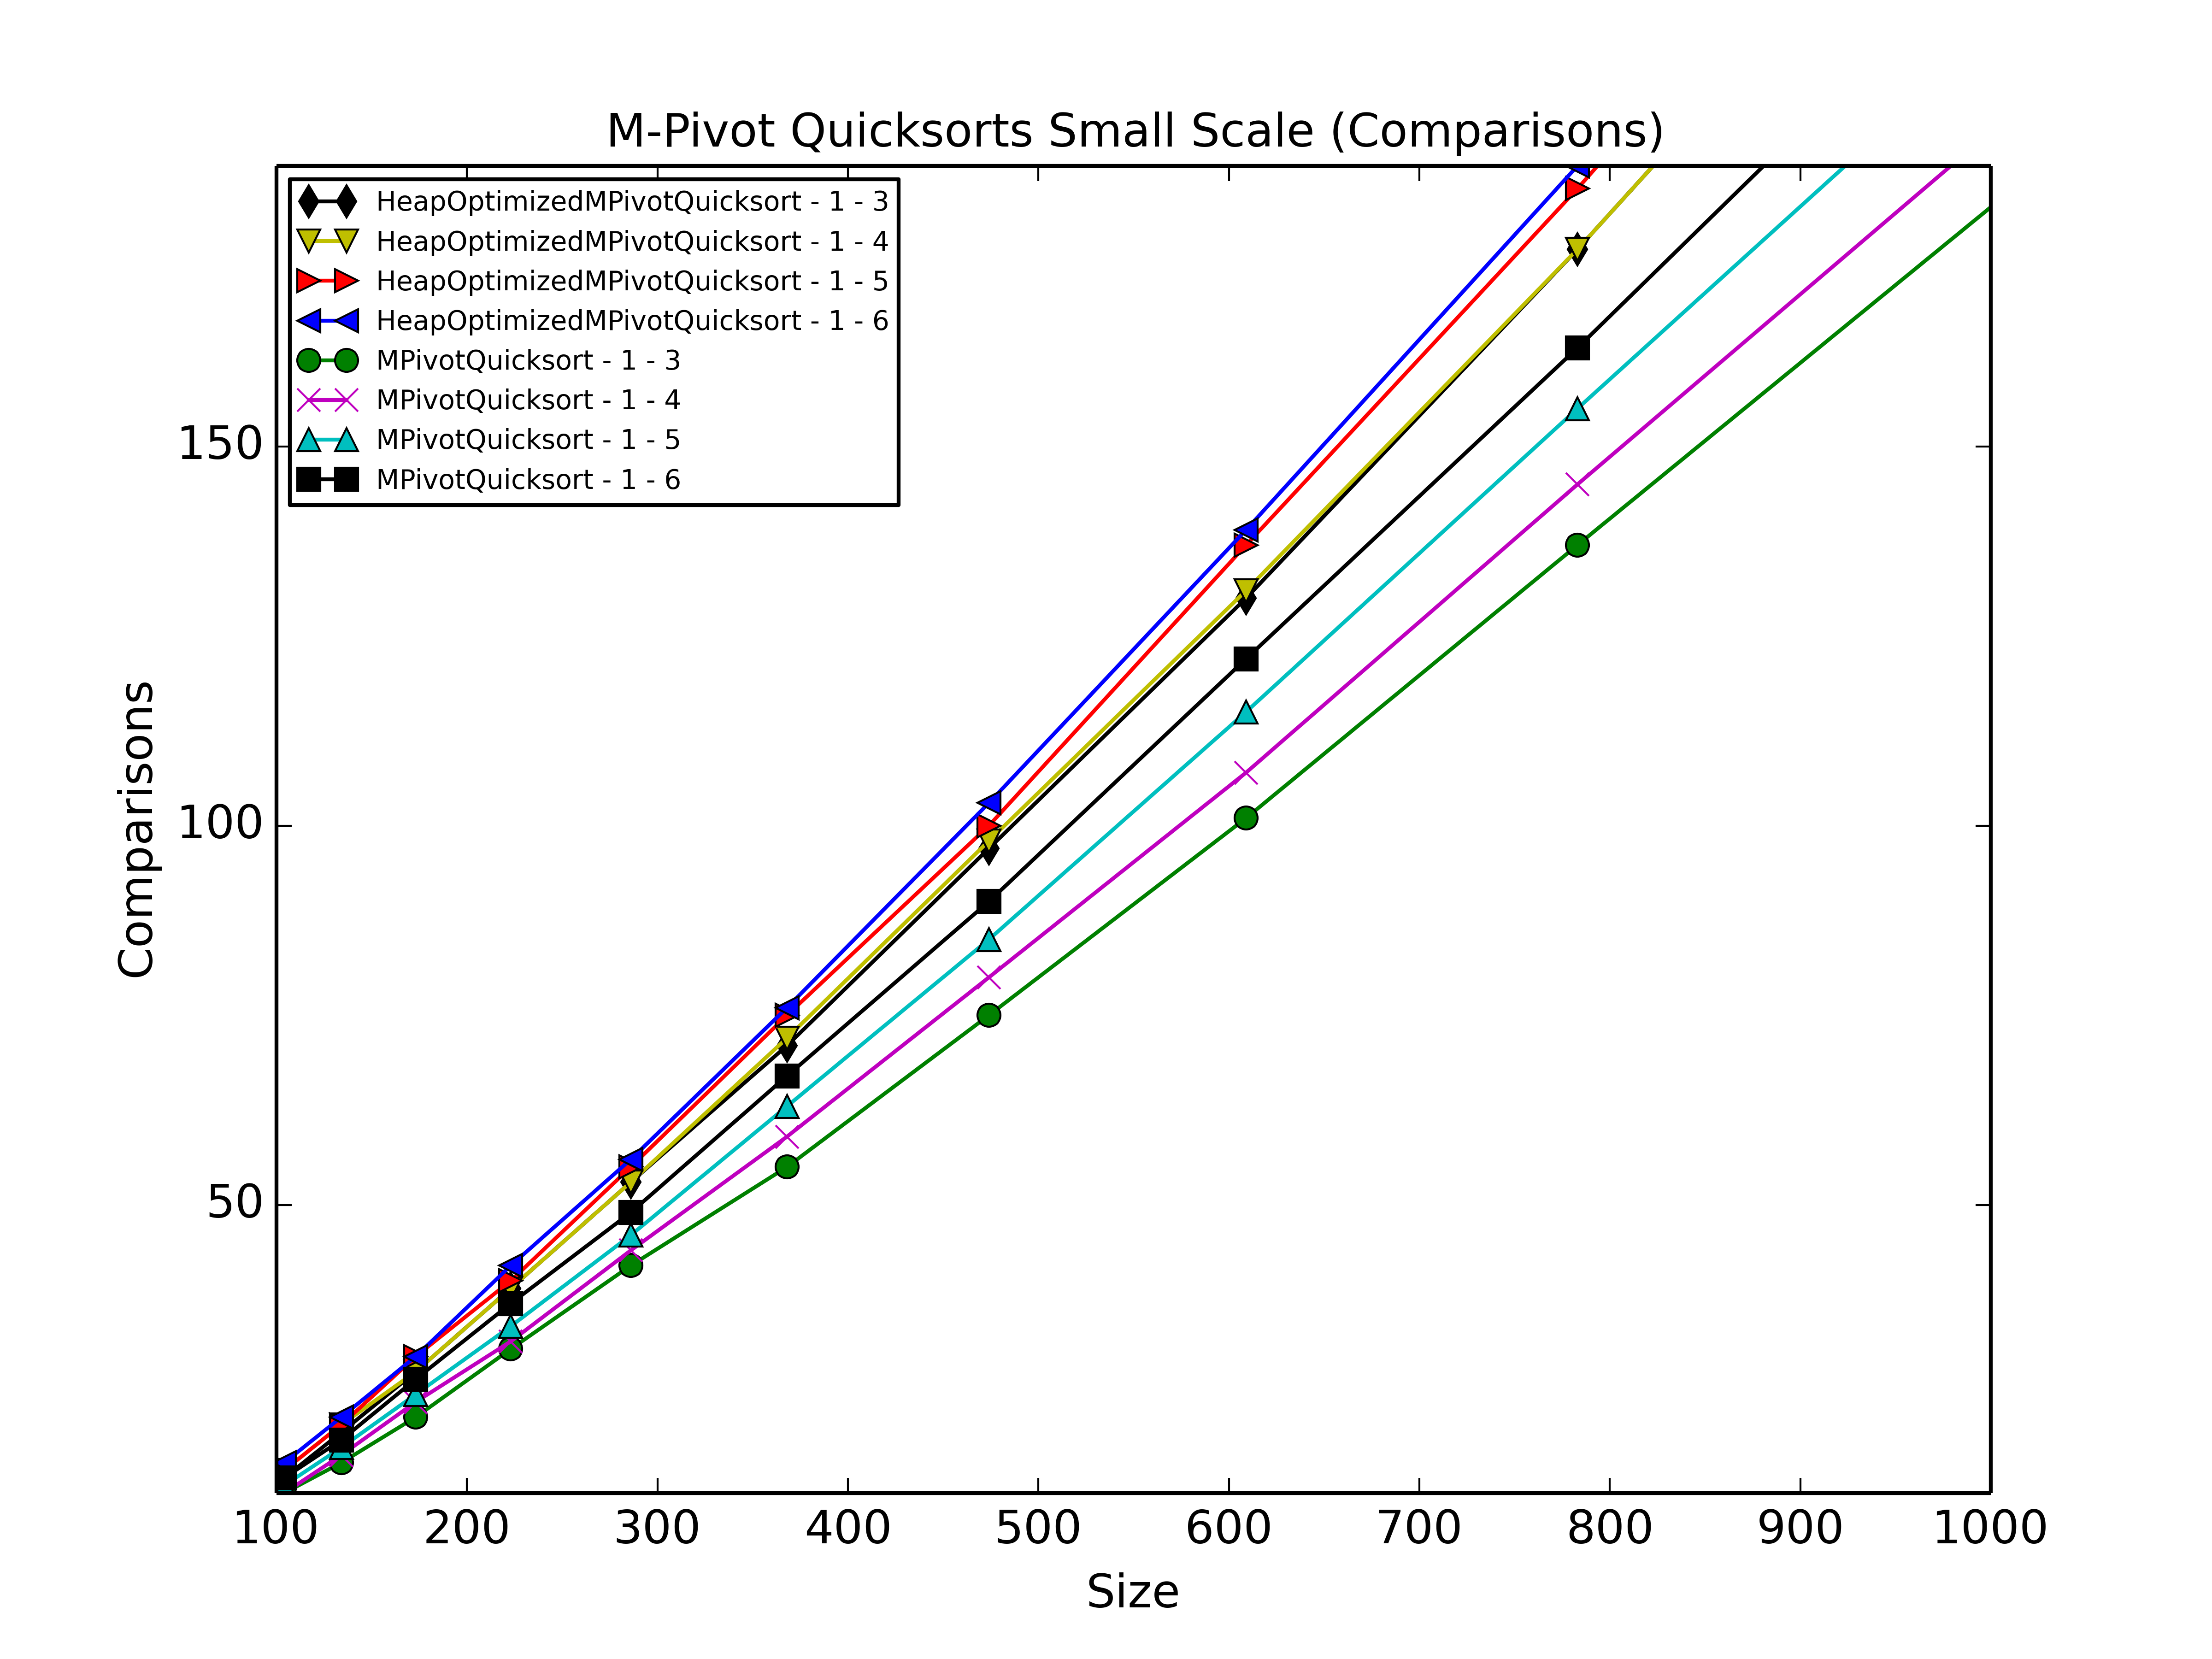
\includegraphics[width=150mm]{M-PivotQuicksortsSmallScale_comp.png}
			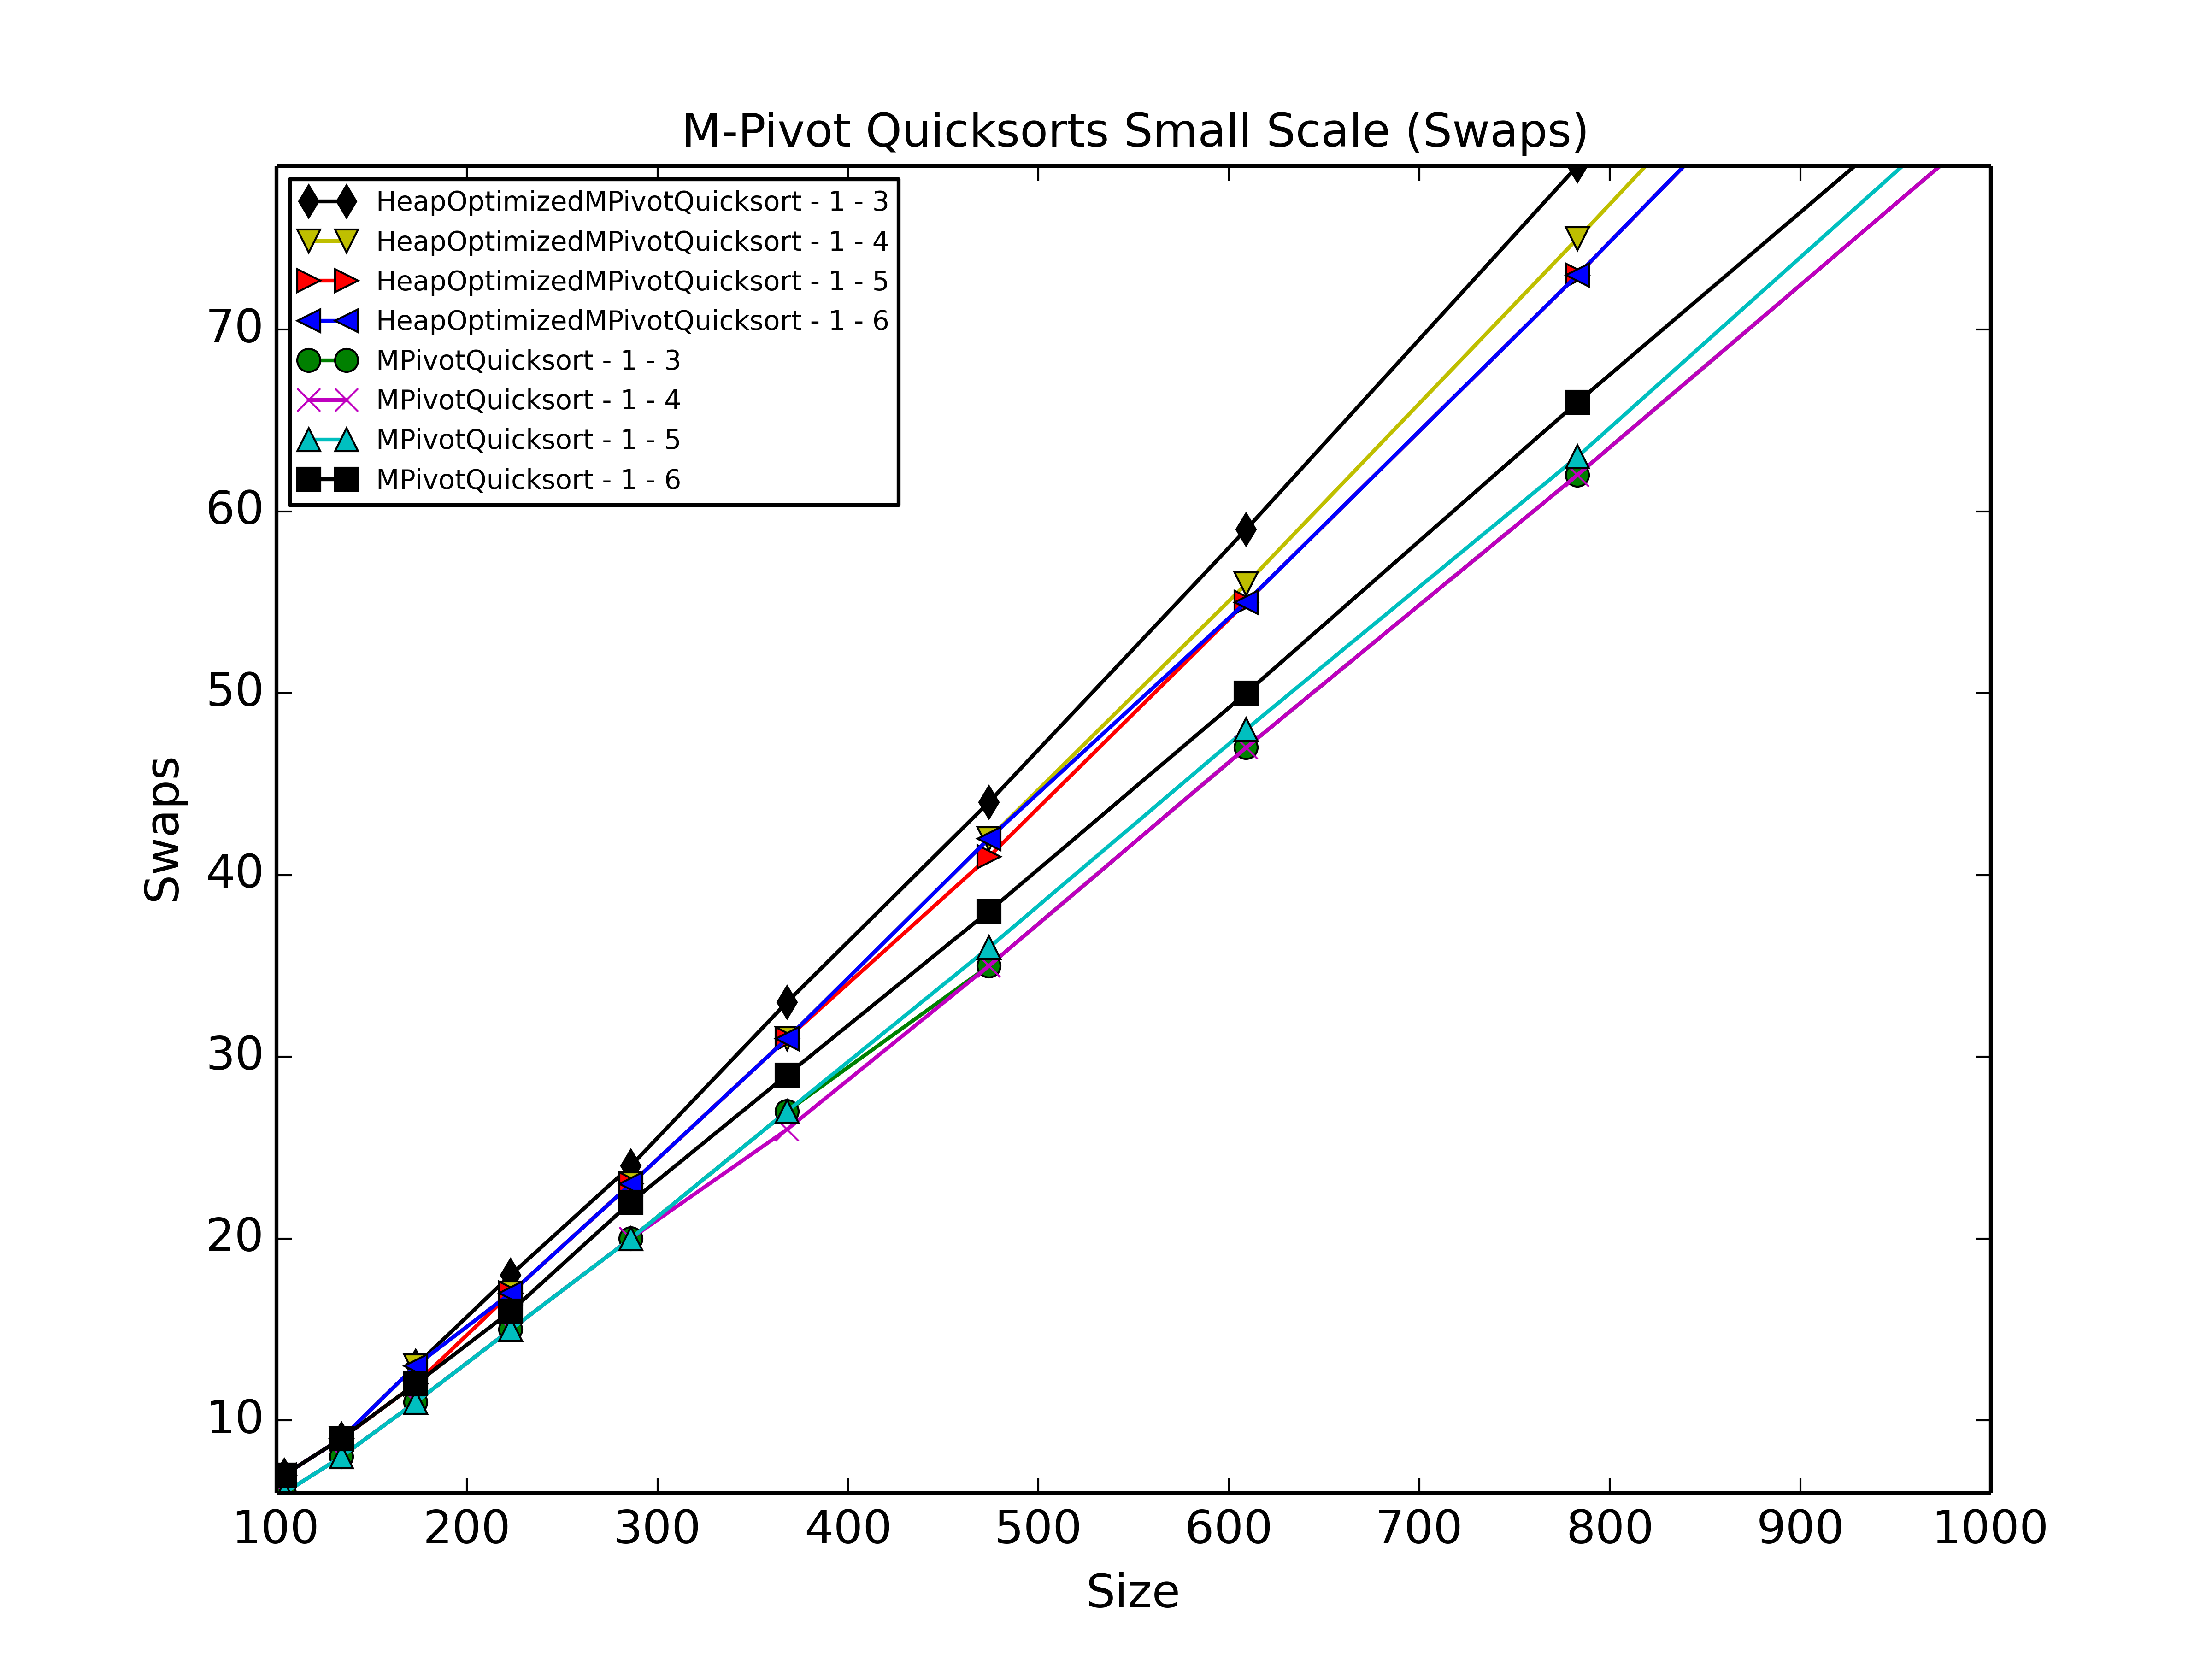
\includegraphics[width=150mm]{M-PivotQuicksortsSmallScale_swap.png}
			\caption{Data from all the version of M-Pivot Sort.}
			\label{fig:MPivot}
		\end{center}
	\end{figure}
